\documentclass[twoside]{book}

% Packages required by doxygen
\usepackage{fixltx2e}
\usepackage{calc}
\usepackage{doxygen}
\usepackage[export]{adjustbox} % also loads graphicx
\usepackage{graphicx}
\usepackage[utf8]{inputenc}
\usepackage{makeidx}
\usepackage{multicol}
\usepackage{multirow}
\PassOptionsToPackage{warn}{textcomp}
\usepackage{textcomp}
\usepackage[nointegrals]{wasysym}
\usepackage[table]{xcolor}

% Font selection
\usepackage[T1]{fontenc}
\usepackage[scaled=.90]{helvet}
\usepackage{courier}
\usepackage{amssymb}
\usepackage{sectsty}
\renewcommand{\familydefault}{\sfdefault}
\allsectionsfont{%
  \fontseries{bc}\selectfont%
  \color{darkgray}%
}
\renewcommand{\DoxyLabelFont}{%
  \fontseries{bc}\selectfont%
  \color{darkgray}%
}
\newcommand{\+}{\discretionary{\mbox{\scriptsize$\hookleftarrow$}}{}{}}

% Page & text layout
\usepackage{geometry}
\geometry{%
  a4paper,%
  top=2.5cm,%
  bottom=2.5cm,%
  left=2.5cm,%
  right=2.5cm%
}
\tolerance=750
\hfuzz=15pt
\hbadness=750
\setlength{\emergencystretch}{15pt}
\setlength{\parindent}{0cm}
\setlength{\parskip}{3ex plus 2ex minus 2ex}
\makeatletter
\renewcommand{\paragraph}{%
  \@startsection{paragraph}{4}{0ex}{-1.0ex}{1.0ex}{%
    \normalfont\normalsize\bfseries\SS@parafont%
  }%
}
\renewcommand{\subparagraph}{%
  \@startsection{subparagraph}{5}{0ex}{-1.0ex}{1.0ex}{%
    \normalfont\normalsize\bfseries\SS@subparafont%
  }%
}
\makeatother

% Headers & footers
\usepackage{fancyhdr}
\pagestyle{fancyplain}
\fancyhead[LE]{\fancyplain{}{\bfseries\thepage}}
\fancyhead[CE]{\fancyplain{}{}}
\fancyhead[RE]{\fancyplain{}{\bfseries\leftmark}}
\fancyhead[LO]{\fancyplain{}{\bfseries\rightmark}}
\fancyhead[CO]{\fancyplain{}{}}
\fancyhead[RO]{\fancyplain{}{\bfseries\thepage}}
\fancyfoot[LE]{\fancyplain{}{}}
\fancyfoot[CE]{\fancyplain{}{}}
\fancyfoot[RE]{\fancyplain{}{\bfseries\scriptsize Generated by Doxygen }}
\fancyfoot[LO]{\fancyplain{}{\bfseries\scriptsize Generated by Doxygen }}
\fancyfoot[CO]{\fancyplain{}{}}
\fancyfoot[RO]{\fancyplain{}{}}
\renewcommand{\footrulewidth}{0.4pt}
\renewcommand{\chaptermark}[1]{%
  \markboth{#1}{}%
}
\renewcommand{\sectionmark}[1]{%
  \markright{\thesection\ #1}%
}

% Indices & bibliography
\usepackage{natbib}
\usepackage[titles]{tocloft}
\setcounter{tocdepth}{3}
\setcounter{secnumdepth}{5}
\makeindex

% Hyperlinks (required, but should be loaded last)
\usepackage{ifpdf}
\ifpdf
  \usepackage[pdftex,pagebackref=true]{hyperref}
\else
  \usepackage[ps2pdf,pagebackref=true]{hyperref}
\fi
\hypersetup{%
  colorlinks=true,%
  linkcolor=blue,%
  citecolor=blue,%
  unicode%
}

% Custom commands
\newcommand{\clearemptydoublepage}{%
  \newpage{\pagestyle{empty}\cleardoublepage}%
}

\usepackage{caption}
\captionsetup{labelsep=space,justification=centering,font={bf},singlelinecheck=off,skip=4pt,position=top}

%===== C O N T E N T S =====

\begin{document}

% Titlepage & ToC
\hypersetup{pageanchor=false,
             bookmarksnumbered=true,
             pdfencoding=unicode
            }
\pagenumbering{alph}
\begin{titlepage}
\vspace*{7cm}
\begin{center}%
{\Large Communication\+Documentation }\\
\vspace*{1cm}
{\large Generated by Doxygen 1.8.14}\\
\end{center}
\end{titlepage}
\clearemptydoublepage
\pagenumbering{roman}
\tableofcontents
\clearemptydoublepage
\pagenumbering{arabic}
\hypersetup{pageanchor=true}

%--- Begin generated contents ---
\chapter{Namespace Index}
\section{Packages}
Here are the packages with brief descriptions (if available)\+:\begin{DoxyCompactList}
\item\contentsline{section}{\mbox{\hyperlink{namespace_application}{Application}} }{\pageref{namespace_application}}{}
\item\contentsline{section}{\mbox{\hyperlink{namespace_application_1_1_controllers}{Application.\+Controllers}} }{\pageref{namespace_application_1_1_controllers}}{}
\item\contentsline{section}{\mbox{\hyperlink{namespace_application_1_1_interfaces}{Application.\+Interfaces}} }{\pageref{namespace_application_1_1_interfaces}}{}
\item\contentsline{section}{\mbox{\hyperlink{namespace_application_1_1_managers}{Application.\+Managers}} }{\pageref{namespace_application_1_1_managers}}{}
\item\contentsline{section}{\mbox{\hyperlink{namespace_application_1_1_misc}{Application.\+Misc}} }{\pageref{namespace_application_1_1_misc}}{}
\end{DoxyCompactList}

\chapter{Hierarchical Index}
\section{Class Hierarchy}
This inheritance list is sorted roughly, but not completely, alphabetically\+:\begin{DoxyCompactList}
\item \contentsline{section}{Application.\+Misc.\+Cache\+List$<$ T\+Class $>$}{\pageref{class_application_1_1_misc_1_1_cache_list}}{}
\item \contentsline{section}{Application.\+Misc.\+Cache\+List$<$ string $>$}{\pageref{class_application_1_1_misc_1_1_cache_list}}{}
\item \contentsline{section}{Application.\+Misc.\+Cache\+List$<$ T\+Class $>$.Contained\+Item}{\pageref{class_application_1_1_misc_1_1_cache_list_1_1_contained_item}}{}
\item Event\+Args\begin{DoxyCompactList}
\item \contentsline{section}{Application.\+Interfaces.\+Timed\+Out\+User\+Event\+Args}{\pageref{class_application_1_1_interfaces_1_1_timed_out_user_event_args}}{}
\end{DoxyCompactList}
\item \contentsline{section}{Application.\+Misc.\+I\+Cache\+Handle}{\pageref{interface_application_1_1_misc_1_1_i_cache_handle}}{}
\item I\+Disposable\begin{DoxyCompactList}
\item \contentsline{section}{Application.\+Misc.\+Smart\+Lock.\+Releaser}{\pageref{struct_application_1_1_misc_1_1_smart_lock_1_1_releaser}}{}
\end{DoxyCompactList}
\item \contentsline{section}{Application.\+Interfaces.\+I\+Game\+Controller}{\pageref{interface_application_1_1_interfaces_1_1_i_game_controller}}{}
\begin{DoxyCompactList}
\item \contentsline{section}{Application.\+Controllers.\+Game\+Controller}{\pageref{class_application_1_1_controllers_1_1_game_controller}}{}
\end{DoxyCompactList}
\item \contentsline{section}{Application.\+Interfaces.\+I\+Lobby\+Controller}{\pageref{interface_application_1_1_interfaces_1_1_i_lobby_controller}}{}
\begin{DoxyCompactList}
\item \contentsline{section}{Application.\+Controllers.\+Lobby\+Controller}{\pageref{class_application_1_1_controllers_1_1_lobby_controller}}{}
\end{DoxyCompactList}
\item \contentsline{section}{Application.\+Interfaces.\+I\+Lobby\+Pool}{\pageref{interface_application_1_1_interfaces_1_1_i_lobby_pool}}{}
\begin{DoxyCompactList}
\item \contentsline{section}{Application.\+Misc.\+Lobby\+Pool}{\pageref{class_application_1_1_misc_1_1_lobby_pool}}{}
\end{DoxyCompactList}
\item \contentsline{section}{Application.\+Interfaces.\+I\+Login\+Manager}{\pageref{interface_application_1_1_interfaces_1_1_i_login_manager}}{}
\begin{DoxyCompactList}
\item \contentsline{section}{Application.\+Managers.\+Login\+Manager}{\pageref{class_application_1_1_managers_1_1_login_manager}}{}
\end{DoxyCompactList}
\item \contentsline{section}{Application.\+Interfaces.\+I\+Timer}{\pageref{interface_application_1_1_interfaces_1_1_i_timer}}{}
\begin{DoxyCompactList}
\item \contentsline{section}{Application.\+Misc.\+Count\+Down\+Timer}{\pageref{class_application_1_1_misc_1_1_count_down_timer}}{}
\end{DoxyCompactList}
\item \contentsline{section}{Application.\+Interfaces.\+I\+User\+Cache}{\pageref{interface_application_1_1_interfaces_1_1_i_user_cache}}{}
\begin{DoxyCompactList}
\item \contentsline{section}{Application.\+Misc.\+User\+Cache}{\pageref{class_application_1_1_misc_1_1_user_cache}}{}
\end{DoxyCompactList}
\item \contentsline{section}{Application.\+Interfaces.\+I\+User\+Controller}{\pageref{interface_application_1_1_interfaces_1_1_i_user_controller}}{}
\begin{DoxyCompactList}
\item \contentsline{section}{Application.\+Controllers.\+User\+Controller}{\pageref{class_application_1_1_controllers_1_1_user_controller}}{}
\end{DoxyCompactList}
\item \contentsline{section}{Application.\+Misc.\+Smart\+Lock}{\pageref{class_application_1_1_misc_1_1_smart_lock}}{}
\end{DoxyCompactList}

\chapter{Class Index}
\section{Class List}
Here are the classes, structs, unions and interfaces with brief descriptions\+:\begin{DoxyCompactList}
\item\contentsline{section}{\mbox{\hyperlink{class_application_1_1_misc_1_1_cache_list}{Application.\+Misc.\+Cache\+List$<$ T\+Class $>$}} }{\pageref{class_application_1_1_misc_1_1_cache_list}}{}
\item\contentsline{section}{\mbox{\hyperlink{class_application_1_1_misc_1_1_cache_list_1_1_contained_item}{Application.\+Misc.\+Cache\+List$<$ T\+Class $>$.\+Contained\+Item}} }{\pageref{class_application_1_1_misc_1_1_cache_list_1_1_contained_item}}{}
\item\contentsline{section}{\mbox{\hyperlink{class_application_1_1_misc_1_1_count_down_timer}{Application.\+Misc.\+Count\+Down\+Timer}} }{\pageref{class_application_1_1_misc_1_1_count_down_timer}}{}
\item\contentsline{section}{\mbox{\hyperlink{class_application_1_1_controllers_1_1_game_controller}{Application.\+Controllers.\+Game\+Controller}} }{\pageref{class_application_1_1_controllers_1_1_game_controller}}{}
\item\contentsline{section}{\mbox{\hyperlink{interface_application_1_1_misc_1_1_i_cache_handle}{Application.\+Misc.\+I\+Cache\+Handle}} }{\pageref{interface_application_1_1_misc_1_1_i_cache_handle}}{}
\item\contentsline{section}{\mbox{\hyperlink{interface_application_1_1_interfaces_1_1_i_game_controller}{Application.\+Interfaces.\+I\+Game\+Controller}} }{\pageref{interface_application_1_1_interfaces_1_1_i_game_controller}}{}
\item\contentsline{section}{\mbox{\hyperlink{interface_application_1_1_interfaces_1_1_i_lobby_controller}{Application.\+Interfaces.\+I\+Lobby\+Controller}} }{\pageref{interface_application_1_1_interfaces_1_1_i_lobby_controller}}{}
\item\contentsline{section}{\mbox{\hyperlink{interface_application_1_1_interfaces_1_1_i_lobby_pool}{Application.\+Interfaces.\+I\+Lobby\+Pool}} }{\pageref{interface_application_1_1_interfaces_1_1_i_lobby_pool}}{}
\item\contentsline{section}{\mbox{\hyperlink{interface_application_1_1_interfaces_1_1_i_login_manager}{Application.\+Interfaces.\+I\+Login\+Manager}} }{\pageref{interface_application_1_1_interfaces_1_1_i_login_manager}}{}
\item\contentsline{section}{\mbox{\hyperlink{interface_application_1_1_interfaces_1_1_i_timer}{Application.\+Interfaces.\+I\+Timer}} }{\pageref{interface_application_1_1_interfaces_1_1_i_timer}}{}
\item\contentsline{section}{\mbox{\hyperlink{interface_application_1_1_interfaces_1_1_i_user_cache}{Application.\+Interfaces.\+I\+User\+Cache}} }{\pageref{interface_application_1_1_interfaces_1_1_i_user_cache}}{}
\item\contentsline{section}{\mbox{\hyperlink{interface_application_1_1_interfaces_1_1_i_user_controller}{Application.\+Interfaces.\+I\+User\+Controller}} }{\pageref{interface_application_1_1_interfaces_1_1_i_user_controller}}{}
\item\contentsline{section}{\mbox{\hyperlink{class_application_1_1_controllers_1_1_lobby_controller}{Application.\+Controllers.\+Lobby\+Controller}} }{\pageref{class_application_1_1_controllers_1_1_lobby_controller}}{}
\item\contentsline{section}{\mbox{\hyperlink{class_application_1_1_misc_1_1_lobby_pool}{Application.\+Misc.\+Lobby\+Pool}} }{\pageref{class_application_1_1_misc_1_1_lobby_pool}}{}
\item\contentsline{section}{\mbox{\hyperlink{class_application_1_1_managers_1_1_login_manager}{Application.\+Managers.\+Login\+Manager}} }{\pageref{class_application_1_1_managers_1_1_login_manager}}{}
\item\contentsline{section}{\mbox{\hyperlink{struct_application_1_1_misc_1_1_smart_lock_1_1_releaser}{Application.\+Misc.\+Smart\+Lock.\+Releaser}} }{\pageref{struct_application_1_1_misc_1_1_smart_lock_1_1_releaser}}{}
\item\contentsline{section}{\mbox{\hyperlink{class_application_1_1_misc_1_1_smart_lock}{Application.\+Misc.\+Smart\+Lock}} \\*Inspired by\+: \href{https://blogs.msdn.microsoft.com/pfxteam/2012/02/12/building-async-coordination-primitives-part-6-asynclock/}{\tt https\+://blogs.\+msdn.\+microsoft.\+com/pfxteam/2012/02/12/building-\/async-\/coordination-\/primitives-\/part-\/6-\/asynclock/} }{\pageref{class_application_1_1_misc_1_1_smart_lock}}{}
\item\contentsline{section}{\mbox{\hyperlink{class_application_1_1_interfaces_1_1_timed_out_user_event_args}{Application.\+Interfaces.\+Timed\+Out\+User\+Event\+Args}} }{\pageref{class_application_1_1_interfaces_1_1_timed_out_user_event_args}}{}
\item\contentsline{section}{\mbox{\hyperlink{class_application_1_1_misc_1_1_user_cache}{Application.\+Misc.\+User\+Cache}} }{\pageref{class_application_1_1_misc_1_1_user_cache}}{}
\item\contentsline{section}{\mbox{\hyperlink{class_application_1_1_controllers_1_1_user_controller}{Application.\+Controllers.\+User\+Controller}} \\*\mbox{\hyperlink{namespace_application}{Application}} User Controller The main purpose of this class is to decouple the framework from our application logic }{\pageref{class_application_1_1_controllers_1_1_user_controller}}{}
\end{DoxyCompactList}

\chapter{File Index}
\section{File List}
Here is a list of all files with brief descriptions\+:\begin{DoxyCompactList}
\item\contentsline{section}{\mbox{\hyperlink{_program_8cs}{Program.\+cs}} }{\pageref{_program_8cs}}{}
\item\contentsline{section}{\mbox{\hyperlink{_startup_8cs}{Startup.\+cs}} }{\pageref{_startup_8cs}}{}
\item\contentsline{section}{Filters/\mbox{\hyperlink{_authorization_swag_attribute_8cs}{Authorization\+Swag\+Attribute.\+cs}} }{\pageref{_authorization_swag_attribute_8cs}}{}
\item\contentsline{section}{Filters/\mbox{\hyperlink{_require_from_query_attribute_8cs}{Require\+From\+Query\+Attribute.\+cs}} }{\pageref{_require_from_query_attribute_8cs}}{}
\item\contentsline{section}{Filters/\mbox{\hyperlink{_validate_model_state_attribute_8cs}{Validate\+Model\+State\+Attribute.\+cs}} }{\pageref{_validate_model_state_attribute_8cs}}{}
\item\contentsline{section}{Formatters/\mbox{\hyperlink{_json_input_formatter_8cs}{Json\+Input\+Formatter.\+cs}} }{\pageref{_json_input_formatter_8cs}}{}
\item\contentsline{section}{Interfaces/\mbox{\hyperlink{_i_lobby_controller_8cs}{I\+Lobby\+Controller.\+cs}} }{\pageref{_i_lobby_controller_8cs}}{}
\item\contentsline{section}{Json\+Serializer\+Extensions/\mbox{\hyperlink{_utility_8cs}{Utility.\+cs}} }{\pageref{_utility_8cs}}{}
\item\contentsline{section}{Model\+Binders(\+Deprecated)/\mbox{\hyperlink{_from_swag_dto_model_binder_8cs}{From\+Swag\+Dto\+Model\+Binder.\+cs}} }{\pageref{_from_swag_dto_model_binder_8cs}}{}
\item\contentsline{section}{Model\+Binders(\+Deprecated)/\+Attributes/\mbox{\hyperlink{_from_swag_dto_attribute_8cs}{From\+Swag\+Dto\+Attribute.\+cs}} }{\pageref{_from_swag_dto_attribute_8cs}}{}
\item\contentsline{section}{Model\+Binders(\+Deprecated)/\+Attributes/\mbox{\hyperlink{_i_from_swag_dto_attribute_8cs}{I\+From\+Swag\+Dto\+Attribute.\+cs}} }{\pageref{_i_from_swag_dto_attribute_8cs}}{}
\item\contentsline{section}{Model\+Binders(\+Deprecated)/\+Value\+Providers/\mbox{\hyperlink{_from_dto_value_provider_8cs}{From\+Dto\+Value\+Provider.\+cs}} }{\pageref{_from_dto_value_provider_8cs}}{}
\item\contentsline{section}{Model\+Binders(\+Deprecated)/\+Value\+Providers/\mbox{\hyperlink{_from_dto_value_provider_factory_8cs}{From\+Dto\+Value\+Provider\+Factory.\+cs}} }{\pageref{_from_dto_value_provider_factory_8cs}}{}
\item\contentsline{section}{obj/\+Debug/netcoreapp2.\+0/\mbox{\hyperlink{_debug_2netcoreapp2_80_2_communication_8_assembly_info_8cs}{Communication.\+Assembly\+Info.\+cs}} }{\pageref{_debug_2netcoreapp2_80_2_communication_8_assembly_info_8cs}}{}
\item\contentsline{section}{obj/\+Release/netcoreapp2.\+0/\mbox{\hyperlink{_release_2netcoreapp2_80_2_communication_8_assembly_info_8cs}{Communication.\+Assembly\+Info.\+cs}} }{\pageref{_release_2netcoreapp2_80_2_communication_8_assembly_info_8cs}}{}
\item\contentsline{section}{R\+E\+S\+T\+Controllers/\mbox{\hyperlink{_lobby_controller_8cs}{Lobby\+Controller.\+cs}} }{\pageref{_lobby_controller_8cs}}{}
\item\contentsline{section}{R\+E\+S\+T\+Controllers/\mbox{\hyperlink{_user_controller_8cs}{User\+Controller.\+cs}} }{\pageref{_user_controller_8cs}}{}
\end{DoxyCompactList}

\chapter{Namespace Documentation}
\hypertarget{namespace_communication}{}\section{Communication Namespace Reference}
\label{namespace_communication}\index{Communication@{Communication}}
\subsection*{Namespaces}
\begin{DoxyCompactItemize}
\item 
namespace \mbox{\hyperlink{namespace_communication_1_1_filters}{Filters}}
\item 
namespace \mbox{\hyperlink{namespace_communication_1_1_formatters}{Formatters}}
\item 
namespace \mbox{\hyperlink{namespace_communication_1_1_interfaces}{Interfaces}}
\item 
namespace \mbox{\hyperlink{namespace_communication_1_1_json_serializer_extensions}{Json\+Serializer\+Extensions}}
\item 
namespace \mbox{\hyperlink{namespace_communication_1_1_model_binders}{Model\+Binders}}
\item 
namespace \mbox{\hyperlink{namespace_communication_1_1_r_e_s_t_controllers}{R\+E\+S\+T\+Controllers}}
\end{DoxyCompactItemize}
\subsection*{Classes}
\begin{DoxyCompactItemize}
\item 
class \mbox{\hyperlink{class_communication_1_1_program}{Program}}
\item 
class \mbox{\hyperlink{class_communication_1_1_startup}{Startup}}
\end{DoxyCompactItemize}

\hypertarget{namespace_communication_1_1_filters}{}\section{Communication.\+Filters Namespace Reference}
\label{namespace_communication_1_1_filters}\index{Communication.\+Filters@{Communication.\+Filters}}
\subsection*{Classes}
\begin{DoxyCompactItemize}
\item 
class \mbox{\hyperlink{class_communication_1_1_filters_1_1_authorization_swag_attribute}{Authorization\+Swag\+Attribute}}
\begin{DoxyCompactList}\small\item\em Provides authentication for requests for Swag Api. Reads username and password from the header of the Http\+Request \end{DoxyCompactList}\item 
class \mbox{\hyperlink{class_communication_1_1_filters_1_1_require_from_query_action_constraint}{Require\+From\+Query\+Action\+Constraint}}
\item 
class \mbox{\hyperlink{class_communication_1_1_filters_1_1_require_from_query_attribute}{Require\+From\+Query\+Attribute}}
\begin{DoxyCompactList}\small\item\em Taken from\+: \href{https://www.strathweb.com/2016/09/required-query-string-parameters-in-asp-net-core-mvc/}{\tt https\+://www.\+strathweb.\+com/2016/09/required-\/query-\/string-\/parameters-\/in-\/asp-\/net-\/core-\/mvc/} \end{DoxyCompactList}\item 
class \mbox{\hyperlink{class_communication_1_1_filters_1_1_validate_model_state_attribute}{Validate\+Model\+State\+Attribute}}
\end{DoxyCompactItemize}

\hypertarget{namespace_communication_1_1_formatters}{}\section{Communication.\+Formatters Namespace Reference}
\label{namespace_communication_1_1_formatters}\index{Communication.\+Formatters@{Communication.\+Formatters}}
\subsection*{Classes}
\begin{DoxyCompactItemize}
\item 
class \mbox{\hyperlink{class_communication_1_1_formatters_1_1_json_input_formatter}{Json\+Input\+Formatter}}
\end{DoxyCompactItemize}

\hypertarget{namespace_communication_1_1_interfaces}{}\section{Communication.\+Interfaces Namespace Reference}
\label{namespace_communication_1_1_interfaces}\index{Communication.\+Interfaces@{Communication.\+Interfaces}}
\subsection*{Classes}
\begin{DoxyCompactItemize}
\item 
interface \mbox{\hyperlink{interface_communication_1_1_interfaces_1_1_i_lobby_controller}{I\+Lobby\+Controller}}
\end{DoxyCompactItemize}

\hypertarget{namespace_communication_1_1_json_serializer_extensions}{}\section{Communication.\+Json\+Serializer\+Extensions Namespace Reference}
\label{namespace_communication_1_1_json_serializer_extensions}\index{Communication.\+Json\+Serializer\+Extensions@{Communication.\+Json\+Serializer\+Extensions}}
\subsection*{Classes}
\begin{DoxyCompactItemize}
\item 
class {\bfseries Utility}
\end{DoxyCompactItemize}

\hypertarget{namespace_communication_1_1_model_binders}{}\section{Communication.\+Model\+Binders Namespace Reference}
\label{namespace_communication_1_1_model_binders}\index{Communication.\+Model\+Binders@{Communication.\+Model\+Binders}}
\subsection*{Namespaces}
\begin{DoxyCompactItemize}
\item 
namespace \mbox{\hyperlink{namespace_communication_1_1_model_binders_1_1_attributes}{Attributes}}
\item 
namespace \mbox{\hyperlink{namespace_communication_1_1_model_binders_1_1_value_providers}{Value\+Providers}}
\end{DoxyCompactItemize}
\subsection*{Classes}
\begin{DoxyCompactItemize}
\item 
class \mbox{\hyperlink{class_communication_1_1_model_binders_1_1_from_swag_dto_model_binder}{From\+Swag\+Dto\+Model\+Binder}}
\begin{DoxyCompactList}\small\item\em Dto to Model converter and binder. The model will bind to the \char`\"{}value\char`\"{} part of a \char`\"{}auth\char`\"{}/\char`\"{}val\char`\"{} request as in accordance with Swag\+Attack Standards \end{DoxyCompactList}\end{DoxyCompactItemize}

\hypertarget{namespace_communication_1_1_model_binders_1_1_attributes}{}\section{Communication.\+Model\+Binders.\+Attributes Namespace Reference}
\label{namespace_communication_1_1_model_binders_1_1_attributes}\index{Communication.\+Model\+Binders.\+Attributes@{Communication.\+Model\+Binders.\+Attributes}}
\subsection*{Classes}
\begin{DoxyCompactItemize}
\item 
class \mbox{\hyperlink{class_communication_1_1_model_binders_1_1_attributes_1_1_from_swag_dto_attribute}{From\+Swag\+Dto\+Attribute}}
\item 
interface \mbox{\hyperlink{interface_communication_1_1_model_binders_1_1_attributes_1_1_i_from_swag_dto_attribute}{I\+From\+Swag\+Dto\+Attribute}}
\end{DoxyCompactItemize}

\hypertarget{namespace_communication_1_1_model_binders_1_1_value_providers}{}\section{Communication.\+Model\+Binders.\+Value\+Providers Namespace Reference}
\label{namespace_communication_1_1_model_binders_1_1_value_providers}\index{Communication.\+Model\+Binders.\+Value\+Providers@{Communication.\+Model\+Binders.\+Value\+Providers}}
\subsection*{Classes}
\begin{DoxyCompactItemize}
\item 
class \mbox{\hyperlink{class_communication_1_1_model_binders_1_1_value_providers_1_1_from_dto_value_provider}{From\+Dto\+Value\+Provider}}
\item 
class \mbox{\hyperlink{class_communication_1_1_model_binders_1_1_value_providers_1_1_from_dto_value_provider_factory}{From\+Dto\+Value\+Provider\+Factory}}
\end{DoxyCompactItemize}

\hypertarget{namespace_communication_1_1_r_e_s_t_controllers}{}\section{Communication.\+R\+E\+S\+T\+Controllers Namespace Reference}
\label{namespace_communication_1_1_r_e_s_t_controllers}\index{Communication.\+R\+E\+S\+T\+Controllers@{Communication.\+R\+E\+S\+T\+Controllers}}
\subsection*{Classes}
\begin{DoxyCompactItemize}
\item 
class \mbox{\hyperlink{class_communication_1_1_r_e_s_t_controllers_1_1_lobby_controller}{Lobby\+Controller}}
\item 
class \mbox{\hyperlink{class_communication_1_1_r_e_s_t_controllers_1_1_user_controller}{User\+Controller}}
\end{DoxyCompactItemize}

\chapter{Class Documentation}
\hypertarget{class_communication_1_1_filters_1_1_authorization_swag_attribute}{}\section{Communication.\+Filters.\+Authorization\+Swag\+Attribute Class Reference}
\label{class_communication_1_1_filters_1_1_authorization_swag_attribute}\index{Communication.\+Filters.\+Authorization\+Swag\+Attribute@{Communication.\+Filters.\+Authorization\+Swag\+Attribute}}


Provides authentication for requests for Swag Api. Reads username and password from the header of the Http\+Request  


Inheritance diagram for Communication.\+Filters.\+Authorization\+Swag\+Attribute\+:\begin{figure}[H]
\begin{center}
\leavevmode
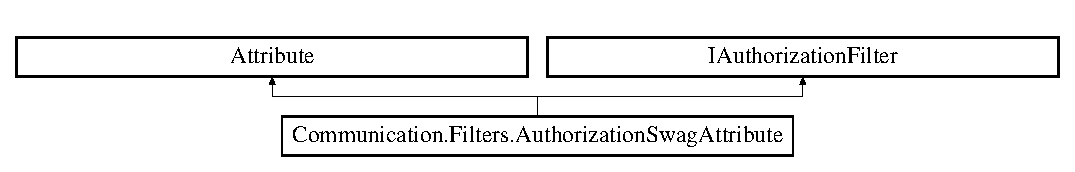
\includegraphics[height=1.866667cm]{class_communication_1_1_filters_1_1_authorization_swag_attribute}
\end{center}
\end{figure}
\subsection*{Public Member Functions}
\begin{DoxyCompactItemize}
\item 
void \mbox{\hyperlink{class_communication_1_1_filters_1_1_authorization_swag_attribute_a0e09022a32fad7c944f5d99ac7486647}{On\+Authorization}} (Authorization\+Filter\+Context context)
\end{DoxyCompactItemize}


\subsection{Detailed Description}
Provides authentication for requests for Swag Api. Reads username and password from the header of the Http\+Request 



\subsection{Member Function Documentation}
\mbox{\Hypertarget{class_communication_1_1_filters_1_1_authorization_swag_attribute_a0e09022a32fad7c944f5d99ac7486647}\label{class_communication_1_1_filters_1_1_authorization_swag_attribute_a0e09022a32fad7c944f5d99ac7486647}} 
\index{Communication\+::\+Filters\+::\+Authorization\+Swag\+Attribute@{Communication\+::\+Filters\+::\+Authorization\+Swag\+Attribute}!On\+Authorization@{On\+Authorization}}
\index{On\+Authorization@{On\+Authorization}!Communication\+::\+Filters\+::\+Authorization\+Swag\+Attribute@{Communication\+::\+Filters\+::\+Authorization\+Swag\+Attribute}}
\subsubsection{\texorpdfstring{On\+Authorization()}{OnAuthorization()}}
{\footnotesize\ttfamily void Communication.\+Filters.\+Authorization\+Swag\+Attribute.\+On\+Authorization (\begin{DoxyParamCaption}\item[{Authorization\+Filter\+Context}]{context }\end{DoxyParamCaption})}



The documentation for this class was generated from the following file\+:\begin{DoxyCompactItemize}
\item 
Filters/\mbox{\hyperlink{_authorization_swag_attribute_8cs}{Authorization\+Swag\+Attribute.\+cs}}\end{DoxyCompactItemize}

\hypertarget{class_communication_1_1_model_binders_1_1_value_providers_1_1_from_dto_value_provider}{}\section{Communication.\+Model\+Binders.\+Value\+Providers.\+From\+Dto\+Value\+Provider Class Reference}
\label{class_communication_1_1_model_binders_1_1_value_providers_1_1_from_dto_value_provider}\index{Communication.\+Model\+Binders.\+Value\+Providers.\+From\+Dto\+Value\+Provider@{Communication.\+Model\+Binders.\+Value\+Providers.\+From\+Dto\+Value\+Provider}}
Inheritance diagram for Communication.\+Model\+Binders.\+Value\+Providers.\+From\+Dto\+Value\+Provider\+:\begin{figure}[H]
\begin{center}
\leavevmode
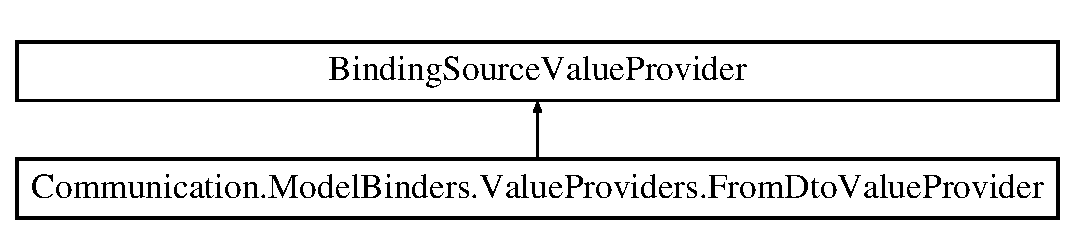
\includegraphics[height=2.000000cm]{class_communication_1_1_model_binders_1_1_value_providers_1_1_from_dto_value_provider}
\end{center}
\end{figure}
\subsection*{Public Member Functions}
\begin{DoxyCompactItemize}
\item 
\mbox{\hyperlink{class_communication_1_1_model_binders_1_1_value_providers_1_1_from_dto_value_provider_a9ddf728279a718c01e6e5903c5b8c016}{From\+Dto\+Value\+Provider}} (object json\+Body, Binding\+Source binding\+Source)
\item 
override bool \mbox{\hyperlink{class_communication_1_1_model_binders_1_1_value_providers_1_1_from_dto_value_provider_a917bbc5d2f3cb896ae8457eb416afae5}{Contains\+Prefix}} (string prefix)
\item 
override Value\+Provider\+Result \mbox{\hyperlink{class_communication_1_1_model_binders_1_1_value_providers_1_1_from_dto_value_provider_a59f5649eff474dd94bf4ce538898272d}{Get\+Value}} (string key)
\end{DoxyCompactItemize}


\subsection{Constructor \& Destructor Documentation}
\mbox{\Hypertarget{class_communication_1_1_model_binders_1_1_value_providers_1_1_from_dto_value_provider_a9ddf728279a718c01e6e5903c5b8c016}\label{class_communication_1_1_model_binders_1_1_value_providers_1_1_from_dto_value_provider_a9ddf728279a718c01e6e5903c5b8c016}} 
\index{Communication\+::\+Model\+Binders\+::\+Value\+Providers\+::\+From\+Dto\+Value\+Provider@{Communication\+::\+Model\+Binders\+::\+Value\+Providers\+::\+From\+Dto\+Value\+Provider}!From\+Dto\+Value\+Provider@{From\+Dto\+Value\+Provider}}
\index{From\+Dto\+Value\+Provider@{From\+Dto\+Value\+Provider}!Communication\+::\+Model\+Binders\+::\+Value\+Providers\+::\+From\+Dto\+Value\+Provider@{Communication\+::\+Model\+Binders\+::\+Value\+Providers\+::\+From\+Dto\+Value\+Provider}}
\subsubsection{\texorpdfstring{From\+Dto\+Value\+Provider()}{FromDtoValueProvider()}}
{\footnotesize\ttfamily Communication.\+Model\+Binders.\+Value\+Providers.\+From\+Dto\+Value\+Provider.\+From\+Dto\+Value\+Provider (\begin{DoxyParamCaption}\item[{object}]{json\+Body,  }\item[{Binding\+Source}]{binding\+Source }\end{DoxyParamCaption})}



\subsection{Member Function Documentation}
\mbox{\Hypertarget{class_communication_1_1_model_binders_1_1_value_providers_1_1_from_dto_value_provider_a917bbc5d2f3cb896ae8457eb416afae5}\label{class_communication_1_1_model_binders_1_1_value_providers_1_1_from_dto_value_provider_a917bbc5d2f3cb896ae8457eb416afae5}} 
\index{Communication\+::\+Model\+Binders\+::\+Value\+Providers\+::\+From\+Dto\+Value\+Provider@{Communication\+::\+Model\+Binders\+::\+Value\+Providers\+::\+From\+Dto\+Value\+Provider}!Contains\+Prefix@{Contains\+Prefix}}
\index{Contains\+Prefix@{Contains\+Prefix}!Communication\+::\+Model\+Binders\+::\+Value\+Providers\+::\+From\+Dto\+Value\+Provider@{Communication\+::\+Model\+Binders\+::\+Value\+Providers\+::\+From\+Dto\+Value\+Provider}}
\subsubsection{\texorpdfstring{Contains\+Prefix()}{ContainsPrefix()}}
{\footnotesize\ttfamily override bool Communication.\+Model\+Binders.\+Value\+Providers.\+From\+Dto\+Value\+Provider.\+Contains\+Prefix (\begin{DoxyParamCaption}\item[{string}]{prefix }\end{DoxyParamCaption})}

\mbox{\Hypertarget{class_communication_1_1_model_binders_1_1_value_providers_1_1_from_dto_value_provider_a59f5649eff474dd94bf4ce538898272d}\label{class_communication_1_1_model_binders_1_1_value_providers_1_1_from_dto_value_provider_a59f5649eff474dd94bf4ce538898272d}} 
\index{Communication\+::\+Model\+Binders\+::\+Value\+Providers\+::\+From\+Dto\+Value\+Provider@{Communication\+::\+Model\+Binders\+::\+Value\+Providers\+::\+From\+Dto\+Value\+Provider}!Get\+Value@{Get\+Value}}
\index{Get\+Value@{Get\+Value}!Communication\+::\+Model\+Binders\+::\+Value\+Providers\+::\+From\+Dto\+Value\+Provider@{Communication\+::\+Model\+Binders\+::\+Value\+Providers\+::\+From\+Dto\+Value\+Provider}}
\subsubsection{\texorpdfstring{Get\+Value()}{GetValue()}}
{\footnotesize\ttfamily override Value\+Provider\+Result Communication.\+Model\+Binders.\+Value\+Providers.\+From\+Dto\+Value\+Provider.\+Get\+Value (\begin{DoxyParamCaption}\item[{string}]{key }\end{DoxyParamCaption})}



The documentation for this class was generated from the following file\+:\begin{DoxyCompactItemize}
\item 
Model\+Binders(\+Deprecated)/\+Value\+Providers/\mbox{\hyperlink{_from_dto_value_provider_8cs}{From\+Dto\+Value\+Provider.\+cs}}\end{DoxyCompactItemize}

\hypertarget{class_communication_1_1_model_binders_1_1_value_providers_1_1_from_dto_value_provider_factory}{}\section{Communication.\+Model\+Binders.\+Value\+Providers.\+From\+Dto\+Value\+Provider\+Factory Class Reference}
\label{class_communication_1_1_model_binders_1_1_value_providers_1_1_from_dto_value_provider_factory}\index{Communication.\+Model\+Binders.\+Value\+Providers.\+From\+Dto\+Value\+Provider\+Factory@{Communication.\+Model\+Binders.\+Value\+Providers.\+From\+Dto\+Value\+Provider\+Factory}}
Inheritance diagram for Communication.\+Model\+Binders.\+Value\+Providers.\+From\+Dto\+Value\+Provider\+Factory\+:\begin{figure}[H]
\begin{center}
\leavevmode
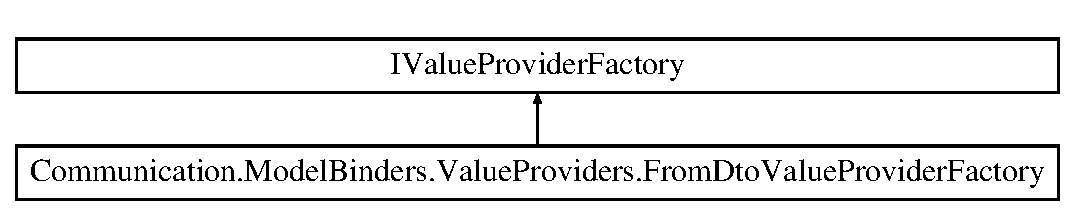
\includegraphics[height=2.000000cm]{class_communication_1_1_model_binders_1_1_value_providers_1_1_from_dto_value_provider_factory}
\end{center}
\end{figure}
\subsection*{Public Member Functions}
\begin{DoxyCompactItemize}
\item 
Task \mbox{\hyperlink{class_communication_1_1_model_binders_1_1_value_providers_1_1_from_dto_value_provider_factory_a66a99cb8b4e1b5a91f8dbe8c50f32fba}{Create\+Value\+Provider\+Async}} (Value\+Provider\+Factory\+Context context)
\end{DoxyCompactItemize}


\subsection{Member Function Documentation}
\mbox{\Hypertarget{class_communication_1_1_model_binders_1_1_value_providers_1_1_from_dto_value_provider_factory_a66a99cb8b4e1b5a91f8dbe8c50f32fba}\label{class_communication_1_1_model_binders_1_1_value_providers_1_1_from_dto_value_provider_factory_a66a99cb8b4e1b5a91f8dbe8c50f32fba}} 
\index{Communication\+::\+Model\+Binders\+::\+Value\+Providers\+::\+From\+Dto\+Value\+Provider\+Factory@{Communication\+::\+Model\+Binders\+::\+Value\+Providers\+::\+From\+Dto\+Value\+Provider\+Factory}!Create\+Value\+Provider\+Async@{Create\+Value\+Provider\+Async}}
\index{Create\+Value\+Provider\+Async@{Create\+Value\+Provider\+Async}!Communication\+::\+Model\+Binders\+::\+Value\+Providers\+::\+From\+Dto\+Value\+Provider\+Factory@{Communication\+::\+Model\+Binders\+::\+Value\+Providers\+::\+From\+Dto\+Value\+Provider\+Factory}}
\subsubsection{\texorpdfstring{Create\+Value\+Provider\+Async()}{CreateValueProviderAsync()}}
{\footnotesize\ttfamily Task Communication.\+Model\+Binders.\+Value\+Providers.\+From\+Dto\+Value\+Provider\+Factory.\+Create\+Value\+Provider\+Async (\begin{DoxyParamCaption}\item[{Value\+Provider\+Factory\+Context}]{context }\end{DoxyParamCaption})}



The documentation for this class was generated from the following file\+:\begin{DoxyCompactItemize}
\item 
Model\+Binders(\+Deprecated)/\+Value\+Providers/\mbox{\hyperlink{_from_dto_value_provider_factory_8cs}{From\+Dto\+Value\+Provider\+Factory.\+cs}}\end{DoxyCompactItemize}

\hypertarget{class_communication_1_1_model_binders_1_1_attributes_1_1_from_swag_dto_attribute}{}\section{Communication.\+Model\+Binders.\+Attributes.\+From\+Swag\+Dto\+Attribute Class Reference}
\label{class_communication_1_1_model_binders_1_1_attributes_1_1_from_swag_dto_attribute}\index{Communication.\+Model\+Binders.\+Attributes.\+From\+Swag\+Dto\+Attribute@{Communication.\+Model\+Binders.\+Attributes.\+From\+Swag\+Dto\+Attribute}}
Inheritance diagram for Communication.\+Model\+Binders.\+Attributes.\+From\+Swag\+Dto\+Attribute\+:\begin{figure}[H]
\begin{center}
\leavevmode
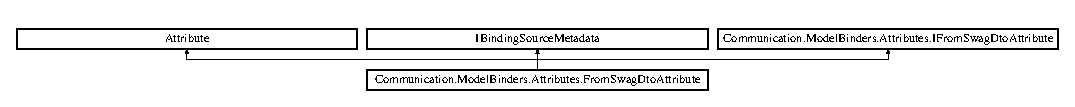
\includegraphics[height=0.990274cm]{class_communication_1_1_model_binders_1_1_attributes_1_1_from_swag_dto_attribute}
\end{center}
\end{figure}
\subsection*{Public Member Functions}
\begin{DoxyCompactItemize}
\item 
\mbox{\hyperlink{class_communication_1_1_model_binders_1_1_attributes_1_1_from_swag_dto_attribute_ae55646bd4c01a2386c3de4b8f80d40e4}{From\+Swag\+Dto\+Attribute}} ()
\end{DoxyCompactItemize}
\subsection*{Public Attributes}
\begin{DoxyCompactItemize}
\item 
Binding\+Source \mbox{\hyperlink{class_communication_1_1_model_binders_1_1_attributes_1_1_from_swag_dto_attribute_ac5a2369f6f9b0bc410d3da81832540d2}{Binding\+Source}} =$>$ Binding\+Source.\+Body
\end{DoxyCompactItemize}
\subsection*{Properties}
\begin{DoxyCompactItemize}
\item 
string \mbox{\hyperlink{class_communication_1_1_model_binders_1_1_attributes_1_1_from_swag_dto_attribute_a3f792d692d2ba7376a1b971127a8c793}{Name}}\hspace{0.3cm}{\ttfamily  \mbox{[}get, set\mbox{]}}
\end{DoxyCompactItemize}


\subsection{Constructor \& Destructor Documentation}
\mbox{\Hypertarget{class_communication_1_1_model_binders_1_1_attributes_1_1_from_swag_dto_attribute_ae55646bd4c01a2386c3de4b8f80d40e4}\label{class_communication_1_1_model_binders_1_1_attributes_1_1_from_swag_dto_attribute_ae55646bd4c01a2386c3de4b8f80d40e4}} 
\index{Communication\+::\+Model\+Binders\+::\+Attributes\+::\+From\+Swag\+Dto\+Attribute@{Communication\+::\+Model\+Binders\+::\+Attributes\+::\+From\+Swag\+Dto\+Attribute}!From\+Swag\+Dto\+Attribute@{From\+Swag\+Dto\+Attribute}}
\index{From\+Swag\+Dto\+Attribute@{From\+Swag\+Dto\+Attribute}!Communication\+::\+Model\+Binders\+::\+Attributes\+::\+From\+Swag\+Dto\+Attribute@{Communication\+::\+Model\+Binders\+::\+Attributes\+::\+From\+Swag\+Dto\+Attribute}}
\subsubsection{\texorpdfstring{From\+Swag\+Dto\+Attribute()}{FromSwagDtoAttribute()}}
{\footnotesize\ttfamily Communication.\+Model\+Binders.\+Attributes.\+From\+Swag\+Dto\+Attribute.\+From\+Swag\+Dto\+Attribute (\begin{DoxyParamCaption}{ }\end{DoxyParamCaption})}



\subsection{Member Data Documentation}
\mbox{\Hypertarget{class_communication_1_1_model_binders_1_1_attributes_1_1_from_swag_dto_attribute_ac5a2369f6f9b0bc410d3da81832540d2}\label{class_communication_1_1_model_binders_1_1_attributes_1_1_from_swag_dto_attribute_ac5a2369f6f9b0bc410d3da81832540d2}} 
\index{Communication\+::\+Model\+Binders\+::\+Attributes\+::\+From\+Swag\+Dto\+Attribute@{Communication\+::\+Model\+Binders\+::\+Attributes\+::\+From\+Swag\+Dto\+Attribute}!Binding\+Source@{Binding\+Source}}
\index{Binding\+Source@{Binding\+Source}!Communication\+::\+Model\+Binders\+::\+Attributes\+::\+From\+Swag\+Dto\+Attribute@{Communication\+::\+Model\+Binders\+::\+Attributes\+::\+From\+Swag\+Dto\+Attribute}}
\subsubsection{\texorpdfstring{Binding\+Source}{BindingSource}}
{\footnotesize\ttfamily Binding\+Source Communication.\+Model\+Binders.\+Attributes.\+From\+Swag\+Dto\+Attribute.\+Binding\+Source =$>$ Binding\+Source.\+Body}



\subsection{Property Documentation}
\mbox{\Hypertarget{class_communication_1_1_model_binders_1_1_attributes_1_1_from_swag_dto_attribute_a3f792d692d2ba7376a1b971127a8c793}\label{class_communication_1_1_model_binders_1_1_attributes_1_1_from_swag_dto_attribute_a3f792d692d2ba7376a1b971127a8c793}} 
\index{Communication\+::\+Model\+Binders\+::\+Attributes\+::\+From\+Swag\+Dto\+Attribute@{Communication\+::\+Model\+Binders\+::\+Attributes\+::\+From\+Swag\+Dto\+Attribute}!Name@{Name}}
\index{Name@{Name}!Communication\+::\+Model\+Binders\+::\+Attributes\+::\+From\+Swag\+Dto\+Attribute@{Communication\+::\+Model\+Binders\+::\+Attributes\+::\+From\+Swag\+Dto\+Attribute}}
\subsubsection{\texorpdfstring{Name}{Name}}
{\footnotesize\ttfamily string Communication.\+Model\+Binders.\+Attributes.\+From\+Swag\+Dto\+Attribute.\+Name\hspace{0.3cm}{\ttfamily [get]}, {\ttfamily [set]}}



The documentation for this class was generated from the following file\+:\begin{DoxyCompactItemize}
\item 
Model\+Binders(\+Deprecated)/\+Attributes/\mbox{\hyperlink{_from_swag_dto_attribute_8cs}{From\+Swag\+Dto\+Attribute.\+cs}}\end{DoxyCompactItemize}

\hypertarget{class_communication_1_1_model_binders_1_1_from_swag_dto_model_binder}{}\section{Communication.\+Model\+Binders.\+From\+Swag\+Dto\+Model\+Binder Class Reference}
\label{class_communication_1_1_model_binders_1_1_from_swag_dto_model_binder}\index{Communication.\+Model\+Binders.\+From\+Swag\+Dto\+Model\+Binder@{Communication.\+Model\+Binders.\+From\+Swag\+Dto\+Model\+Binder}}


Dto to Model converter and binder. The model will bind to the \char`\"{}value\char`\"{} part of a \char`\"{}auth\char`\"{}/\char`\"{}val\char`\"{} request as in accordance with Swag\+Attack Standards  


Inheritance diagram for Communication.\+Model\+Binders.\+From\+Swag\+Dto\+Model\+Binder\+:\begin{figure}[H]
\begin{center}
\leavevmode
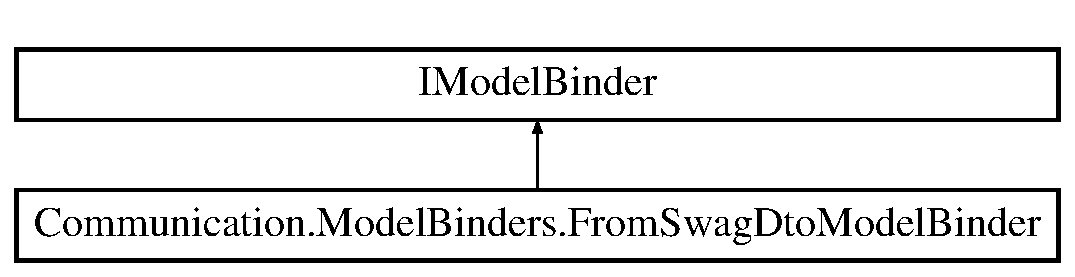
\includegraphics[height=2.000000cm]{class_communication_1_1_model_binders_1_1_from_swag_dto_model_binder}
\end{center}
\end{figure}
\subsection*{Public Member Functions}
\begin{DoxyCompactItemize}
\item 
async Task \mbox{\hyperlink{class_communication_1_1_model_binders_1_1_from_swag_dto_model_binder_a9f06cf186abe70ff88cf3895a5d83719}{Bind\+Model\+Async}} (Model\+Binding\+Context binding\+Context)
\end{DoxyCompactItemize}


\subsection{Detailed Description}
Dto to Model converter and binder. The model will bind to the \char`\"{}value\char`\"{} part of a \char`\"{}auth\char`\"{}/\char`\"{}val\char`\"{} request as in accordance with Swag\+Attack Standards 



\subsection{Member Function Documentation}
\mbox{\Hypertarget{class_communication_1_1_model_binders_1_1_from_swag_dto_model_binder_a9f06cf186abe70ff88cf3895a5d83719}\label{class_communication_1_1_model_binders_1_1_from_swag_dto_model_binder_a9f06cf186abe70ff88cf3895a5d83719}} 
\index{Communication\+::\+Model\+Binders\+::\+From\+Swag\+Dto\+Model\+Binder@{Communication\+::\+Model\+Binders\+::\+From\+Swag\+Dto\+Model\+Binder}!Bind\+Model\+Async@{Bind\+Model\+Async}}
\index{Bind\+Model\+Async@{Bind\+Model\+Async}!Communication\+::\+Model\+Binders\+::\+From\+Swag\+Dto\+Model\+Binder@{Communication\+::\+Model\+Binders\+::\+From\+Swag\+Dto\+Model\+Binder}}
\subsubsection{\texorpdfstring{Bind\+Model\+Async()}{BindModelAsync()}}
{\footnotesize\ttfamily async Task Communication.\+Model\+Binders.\+From\+Swag\+Dto\+Model\+Binder.\+Bind\+Model\+Async (\begin{DoxyParamCaption}\item[{Model\+Binding\+Context}]{binding\+Context }\end{DoxyParamCaption})}



The documentation for this class was generated from the following file\+:\begin{DoxyCompactItemize}
\item 
Model\+Binders(\+Deprecated)/\mbox{\hyperlink{_from_swag_dto_model_binder_8cs}{From\+Swag\+Dto\+Model\+Binder.\+cs}}\end{DoxyCompactItemize}

\hypertarget{interface_communication_1_1_model_binders_1_1_attributes_1_1_i_from_swag_dto_attribute}{}\section{Communication.\+Model\+Binders.\+Attributes.\+I\+From\+Swag\+Dto\+Attribute Interface Reference}
\label{interface_communication_1_1_model_binders_1_1_attributes_1_1_i_from_swag_dto_attribute}\index{Communication.\+Model\+Binders.\+Attributes.\+I\+From\+Swag\+Dto\+Attribute@{Communication.\+Model\+Binders.\+Attributes.\+I\+From\+Swag\+Dto\+Attribute}}
Inheritance diagram for Communication.\+Model\+Binders.\+Attributes.\+I\+From\+Swag\+Dto\+Attribute\+:\begin{figure}[H]
\begin{center}
\leavevmode
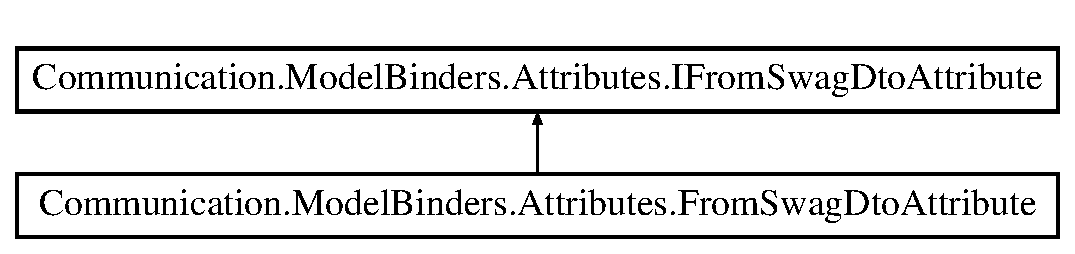
\includegraphics[height=2.000000cm]{interface_communication_1_1_model_binders_1_1_attributes_1_1_i_from_swag_dto_attribute}
\end{center}
\end{figure}
\subsection*{Properties}
\begin{DoxyCompactItemize}
\item 
string \mbox{\hyperlink{interface_communication_1_1_model_binders_1_1_attributes_1_1_i_from_swag_dto_attribute_a7d6647dfb2d0e32ea5721206c20316c3}{Name}}\hspace{0.3cm}{\ttfamily  \mbox{[}get, set\mbox{]}}
\end{DoxyCompactItemize}


\subsection{Property Documentation}
\mbox{\Hypertarget{interface_communication_1_1_model_binders_1_1_attributes_1_1_i_from_swag_dto_attribute_a7d6647dfb2d0e32ea5721206c20316c3}\label{interface_communication_1_1_model_binders_1_1_attributes_1_1_i_from_swag_dto_attribute_a7d6647dfb2d0e32ea5721206c20316c3}} 
\index{Communication\+::\+Model\+Binders\+::\+Attributes\+::\+I\+From\+Swag\+Dto\+Attribute@{Communication\+::\+Model\+Binders\+::\+Attributes\+::\+I\+From\+Swag\+Dto\+Attribute}!Name@{Name}}
\index{Name@{Name}!Communication\+::\+Model\+Binders\+::\+Attributes\+::\+I\+From\+Swag\+Dto\+Attribute@{Communication\+::\+Model\+Binders\+::\+Attributes\+::\+I\+From\+Swag\+Dto\+Attribute}}
\subsubsection{\texorpdfstring{Name}{Name}}
{\footnotesize\ttfamily string Communication.\+Model\+Binders.\+Attributes.\+I\+From\+Swag\+Dto\+Attribute.\+Name\hspace{0.3cm}{\ttfamily [get]}, {\ttfamily [set]}}



The documentation for this interface was generated from the following file\+:\begin{DoxyCompactItemize}
\item 
Model\+Binders(\+Deprecated)/\+Attributes/\mbox{\hyperlink{_i_from_swag_dto_attribute_8cs}{I\+From\+Swag\+Dto\+Attribute.\+cs}}\end{DoxyCompactItemize}

\hypertarget{interface_communication_1_1_interfaces_1_1_i_lobby_controller}{}\section{Communication.\+Interfaces.\+I\+Lobby\+Controller Interface Reference}
\label{interface_communication_1_1_interfaces_1_1_i_lobby_controller}\index{Communication.\+Interfaces.\+I\+Lobby\+Controller@{Communication.\+Interfaces.\+I\+Lobby\+Controller}}
\subsection*{Public Member Functions}
\begin{DoxyCompactItemize}
\item 
I\+Action\+Result \mbox{\hyperlink{interface_communication_1_1_interfaces_1_1_i_lobby_controller_a68e8088f8e43f261906c74604ada45b8}{Get\+All\+Lobbies}} ()
\item 
I\+Action\+Result \mbox{\hyperlink{interface_communication_1_1_interfaces_1_1_i_lobby_controller_aed4c7c417faceb72a7e8248728c3a271}{Get\+Lobby}} (string lobby\+Id)
\item 
I\+Action\+Result \mbox{\hyperlink{interface_communication_1_1_interfaces_1_1_i_lobby_controller_a79179036a5010d2f64ce09c0ac67520f}{Create\+Lobby}} (string lobby\+Id, string username)
\item 
I\+Action\+Result \mbox{\hyperlink{interface_communication_1_1_interfaces_1_1_i_lobby_controller_a66b8bdd9794da0454cac2e6aba9b4faf}{Leave\+Lobby}} (string lobby\+Id, string username)
\item 
I\+Action\+Result \mbox{\hyperlink{interface_communication_1_1_interfaces_1_1_i_lobby_controller_aaf8bea84ae5b4d36abe14fc305b055f2}{Join\+Lobby}} (string lobby\+Id, string username)
\end{DoxyCompactItemize}


\subsection{Member Function Documentation}
\mbox{\Hypertarget{interface_communication_1_1_interfaces_1_1_i_lobby_controller_a79179036a5010d2f64ce09c0ac67520f}\label{interface_communication_1_1_interfaces_1_1_i_lobby_controller_a79179036a5010d2f64ce09c0ac67520f}} 
\index{Communication\+::\+Interfaces\+::\+I\+Lobby\+Controller@{Communication\+::\+Interfaces\+::\+I\+Lobby\+Controller}!Create\+Lobby@{Create\+Lobby}}
\index{Create\+Lobby@{Create\+Lobby}!Communication\+::\+Interfaces\+::\+I\+Lobby\+Controller@{Communication\+::\+Interfaces\+::\+I\+Lobby\+Controller}}
\subsubsection{\texorpdfstring{Create\+Lobby()}{CreateLobby()}}
{\footnotesize\ttfamily I\+Action\+Result Communication.\+Interfaces.\+I\+Lobby\+Controller.\+Create\+Lobby (\begin{DoxyParamCaption}\item[{string}]{lobby\+Id,  }\item[{string}]{username }\end{DoxyParamCaption})}

\mbox{\Hypertarget{interface_communication_1_1_interfaces_1_1_i_lobby_controller_a68e8088f8e43f261906c74604ada45b8}\label{interface_communication_1_1_interfaces_1_1_i_lobby_controller_a68e8088f8e43f261906c74604ada45b8}} 
\index{Communication\+::\+Interfaces\+::\+I\+Lobby\+Controller@{Communication\+::\+Interfaces\+::\+I\+Lobby\+Controller}!Get\+All\+Lobbies@{Get\+All\+Lobbies}}
\index{Get\+All\+Lobbies@{Get\+All\+Lobbies}!Communication\+::\+Interfaces\+::\+I\+Lobby\+Controller@{Communication\+::\+Interfaces\+::\+I\+Lobby\+Controller}}
\subsubsection{\texorpdfstring{Get\+All\+Lobbies()}{GetAllLobbies()}}
{\footnotesize\ttfamily I\+Action\+Result Communication.\+Interfaces.\+I\+Lobby\+Controller.\+Get\+All\+Lobbies (\begin{DoxyParamCaption}{ }\end{DoxyParamCaption})}

\mbox{\Hypertarget{interface_communication_1_1_interfaces_1_1_i_lobby_controller_aed4c7c417faceb72a7e8248728c3a271}\label{interface_communication_1_1_interfaces_1_1_i_lobby_controller_aed4c7c417faceb72a7e8248728c3a271}} 
\index{Communication\+::\+Interfaces\+::\+I\+Lobby\+Controller@{Communication\+::\+Interfaces\+::\+I\+Lobby\+Controller}!Get\+Lobby@{Get\+Lobby}}
\index{Get\+Lobby@{Get\+Lobby}!Communication\+::\+Interfaces\+::\+I\+Lobby\+Controller@{Communication\+::\+Interfaces\+::\+I\+Lobby\+Controller}}
\subsubsection{\texorpdfstring{Get\+Lobby()}{GetLobby()}}
{\footnotesize\ttfamily I\+Action\+Result Communication.\+Interfaces.\+I\+Lobby\+Controller.\+Get\+Lobby (\begin{DoxyParamCaption}\item[{string}]{lobby\+Id }\end{DoxyParamCaption})}

\mbox{\Hypertarget{interface_communication_1_1_interfaces_1_1_i_lobby_controller_aaf8bea84ae5b4d36abe14fc305b055f2}\label{interface_communication_1_1_interfaces_1_1_i_lobby_controller_aaf8bea84ae5b4d36abe14fc305b055f2}} 
\index{Communication\+::\+Interfaces\+::\+I\+Lobby\+Controller@{Communication\+::\+Interfaces\+::\+I\+Lobby\+Controller}!Join\+Lobby@{Join\+Lobby}}
\index{Join\+Lobby@{Join\+Lobby}!Communication\+::\+Interfaces\+::\+I\+Lobby\+Controller@{Communication\+::\+Interfaces\+::\+I\+Lobby\+Controller}}
\subsubsection{\texorpdfstring{Join\+Lobby()}{JoinLobby()}}
{\footnotesize\ttfamily I\+Action\+Result Communication.\+Interfaces.\+I\+Lobby\+Controller.\+Join\+Lobby (\begin{DoxyParamCaption}\item[{string}]{lobby\+Id,  }\item[{string}]{username }\end{DoxyParamCaption})}

\mbox{\Hypertarget{interface_communication_1_1_interfaces_1_1_i_lobby_controller_a66b8bdd9794da0454cac2e6aba9b4faf}\label{interface_communication_1_1_interfaces_1_1_i_lobby_controller_a66b8bdd9794da0454cac2e6aba9b4faf}} 
\index{Communication\+::\+Interfaces\+::\+I\+Lobby\+Controller@{Communication\+::\+Interfaces\+::\+I\+Lobby\+Controller}!Leave\+Lobby@{Leave\+Lobby}}
\index{Leave\+Lobby@{Leave\+Lobby}!Communication\+::\+Interfaces\+::\+I\+Lobby\+Controller@{Communication\+::\+Interfaces\+::\+I\+Lobby\+Controller}}
\subsubsection{\texorpdfstring{Leave\+Lobby()}{LeaveLobby()}}
{\footnotesize\ttfamily I\+Action\+Result Communication.\+Interfaces.\+I\+Lobby\+Controller.\+Leave\+Lobby (\begin{DoxyParamCaption}\item[{string}]{lobby\+Id,  }\item[{string}]{username }\end{DoxyParamCaption})}



The documentation for this interface was generated from the following file\+:\begin{DoxyCompactItemize}
\item 
Interfaces/\mbox{\hyperlink{_i_lobby_controller_8cs}{I\+Lobby\+Controller.\+cs}}\end{DoxyCompactItemize}

\hypertarget{class_communication_1_1_formatters_1_1_json_input_formatter}{}\section{Communication.\+Formatters.\+Json\+Input\+Formatter Class Reference}
\label{class_communication_1_1_formatters_1_1_json_input_formatter}\index{Communication.\+Formatters.\+Json\+Input\+Formatter@{Communication.\+Formatters.\+Json\+Input\+Formatter}}
Inheritance diagram for Communication.\+Formatters.\+Json\+Input\+Formatter\+:\begin{figure}[H]
\begin{center}
\leavevmode
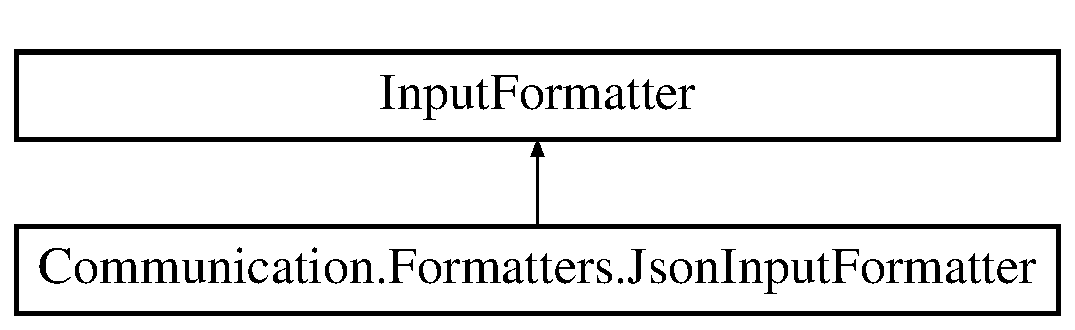
\includegraphics[height=2.000000cm]{class_communication_1_1_formatters_1_1_json_input_formatter}
\end{center}
\end{figure}
\subsection*{Public Member Functions}
\begin{DoxyCompactItemize}
\item 
override bool \mbox{\hyperlink{class_communication_1_1_formatters_1_1_json_input_formatter_a7e9bfac22f7e8b5c8e9b890c992109bb}{Can\+Read}} (Input\+Formatter\+Context context)
\item 
override async Task$<$ Input\+Formatter\+Result $>$ \mbox{\hyperlink{class_communication_1_1_formatters_1_1_json_input_formatter_a419451e6045e0c5ebca0d71496437c21}{Read\+Request\+Body\+Async}} (Input\+Formatter\+Context context)
\end{DoxyCompactItemize}


\subsection{Member Function Documentation}
\mbox{\Hypertarget{class_communication_1_1_formatters_1_1_json_input_formatter_a7e9bfac22f7e8b5c8e9b890c992109bb}\label{class_communication_1_1_formatters_1_1_json_input_formatter_a7e9bfac22f7e8b5c8e9b890c992109bb}} 
\index{Communication\+::\+Formatters\+::\+Json\+Input\+Formatter@{Communication\+::\+Formatters\+::\+Json\+Input\+Formatter}!Can\+Read@{Can\+Read}}
\index{Can\+Read@{Can\+Read}!Communication\+::\+Formatters\+::\+Json\+Input\+Formatter@{Communication\+::\+Formatters\+::\+Json\+Input\+Formatter}}
\subsubsection{\texorpdfstring{Can\+Read()}{CanRead()}}
{\footnotesize\ttfamily override bool Communication.\+Formatters.\+Json\+Input\+Formatter.\+Can\+Read (\begin{DoxyParamCaption}\item[{Input\+Formatter\+Context}]{context }\end{DoxyParamCaption})}

\mbox{\Hypertarget{class_communication_1_1_formatters_1_1_json_input_formatter_a419451e6045e0c5ebca0d71496437c21}\label{class_communication_1_1_formatters_1_1_json_input_formatter_a419451e6045e0c5ebca0d71496437c21}} 
\index{Communication\+::\+Formatters\+::\+Json\+Input\+Formatter@{Communication\+::\+Formatters\+::\+Json\+Input\+Formatter}!Read\+Request\+Body\+Async@{Read\+Request\+Body\+Async}}
\index{Read\+Request\+Body\+Async@{Read\+Request\+Body\+Async}!Communication\+::\+Formatters\+::\+Json\+Input\+Formatter@{Communication\+::\+Formatters\+::\+Json\+Input\+Formatter}}
\subsubsection{\texorpdfstring{Read\+Request\+Body\+Async()}{ReadRequestBodyAsync()}}
{\footnotesize\ttfamily override async Task$<$Input\+Formatter\+Result$>$ Communication.\+Formatters.\+Json\+Input\+Formatter.\+Read\+Request\+Body\+Async (\begin{DoxyParamCaption}\item[{Input\+Formatter\+Context}]{context }\end{DoxyParamCaption})}



The documentation for this class was generated from the following file\+:\begin{DoxyCompactItemize}
\item 
Formatters/\mbox{\hyperlink{_json_input_formatter_8cs}{Json\+Input\+Formatter.\+cs}}\end{DoxyCompactItemize}

\hypertarget{class_communication_1_1_r_e_s_t_controllers_1_1_lobby_controller}{}\section{Communication.\+R\+E\+S\+T\+Controllers.\+Lobby\+Controller Class Reference}
\label{class_communication_1_1_r_e_s_t_controllers_1_1_lobby_controller}\index{Communication.\+R\+E\+S\+T\+Controllers.\+Lobby\+Controller@{Communication.\+R\+E\+S\+T\+Controllers.\+Lobby\+Controller}}
Inheritance diagram for Communication.\+R\+E\+S\+T\+Controllers.\+Lobby\+Controller\+:\begin{figure}[H]
\begin{center}
\leavevmode
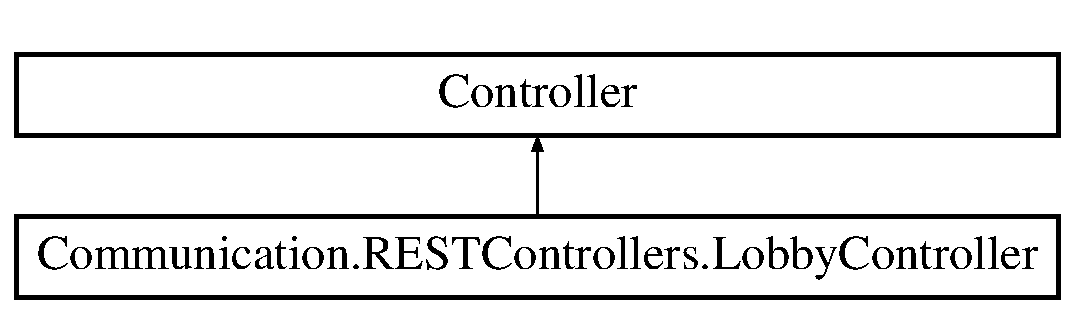
\includegraphics[height=2.000000cm]{class_communication_1_1_r_e_s_t_controllers_1_1_lobby_controller}
\end{center}
\end{figure}
\subsection*{Public Member Functions}
\begin{DoxyCompactItemize}
\item 
\mbox{\hyperlink{class_communication_1_1_r_e_s_t_controllers_1_1_lobby_controller_a6966ace5382d916c0f9a9cada92aef71}{Lobby\+Controller}} (Application.\+Interfaces.\+I\+Lobby\+Controller lobby\+Controller)
\item 
async Task$<$ I\+Action\+Result $>$ \mbox{\hyperlink{class_communication_1_1_r_e_s_t_controllers_1_1_lobby_controller_a38e3aa49bd452dee823bd25bbfacef9f}{Get\+Lobby\+Async}} (string lobby\+Id)
\item 
async Task$<$ I\+Action\+Result $>$ \mbox{\hyperlink{class_communication_1_1_r_e_s_t_controllers_1_1_lobby_controller_a06d83adbec30fc919a2c69e0c3360ac0}{Get\+All\+Lobbies\+Async}} ()
\item 
async Task$<$ I\+Action\+Result $>$ \mbox{\hyperlink{class_communication_1_1_r_e_s_t_controllers_1_1_lobby_controller_a30bcfcd718a55e8c413f61d38d176ef8}{Join\+Lobby\+Async}} (\mbox{[}From\+Query\mbox{]}string lobby\+Id, \mbox{[}From\+Header\mbox{]} string username)
\item 
async Task$<$ I\+Action\+Result $>$ \mbox{\hyperlink{class_communication_1_1_r_e_s_t_controllers_1_1_lobby_controller_a85eeb02c29c53fd63d6a5d1765128854}{Leave\+Lobby\+Async}} (\mbox{[}From\+Query\mbox{]}string lobby\+Id, \mbox{[}From\+Header\mbox{]} string username)
\item 
async Task$<$ I\+Action\+Result $>$ \mbox{\hyperlink{class_communication_1_1_r_e_s_t_controllers_1_1_lobby_controller_a4586b9012b563d032cccc9d48049f6fb}{Create\+Lobby\+Async}} (\mbox{[}From\+Query\mbox{]}string lobby\+Id, \mbox{[}From\+Header\mbox{]} string username)
\end{DoxyCompactItemize}


\subsection{Constructor \& Destructor Documentation}
\mbox{\Hypertarget{class_communication_1_1_r_e_s_t_controllers_1_1_lobby_controller_a6966ace5382d916c0f9a9cada92aef71}\label{class_communication_1_1_r_e_s_t_controllers_1_1_lobby_controller_a6966ace5382d916c0f9a9cada92aef71}} 
\index{Communication\+::\+R\+E\+S\+T\+Controllers\+::\+Lobby\+Controller@{Communication\+::\+R\+E\+S\+T\+Controllers\+::\+Lobby\+Controller}!Lobby\+Controller@{Lobby\+Controller}}
\index{Lobby\+Controller@{Lobby\+Controller}!Communication\+::\+R\+E\+S\+T\+Controllers\+::\+Lobby\+Controller@{Communication\+::\+R\+E\+S\+T\+Controllers\+::\+Lobby\+Controller}}
\subsubsection{\texorpdfstring{Lobby\+Controller()}{LobbyController()}}
{\footnotesize\ttfamily Communication.\+R\+E\+S\+T\+Controllers.\+Lobby\+Controller.\+Lobby\+Controller (\begin{DoxyParamCaption}\item[{Application.\+Interfaces.\+I\+Lobby\+Controller}]{lobby\+Controller }\end{DoxyParamCaption})}



\subsection{Member Function Documentation}
\mbox{\Hypertarget{class_communication_1_1_r_e_s_t_controllers_1_1_lobby_controller_a4586b9012b563d032cccc9d48049f6fb}\label{class_communication_1_1_r_e_s_t_controllers_1_1_lobby_controller_a4586b9012b563d032cccc9d48049f6fb}} 
\index{Communication\+::\+R\+E\+S\+T\+Controllers\+::\+Lobby\+Controller@{Communication\+::\+R\+E\+S\+T\+Controllers\+::\+Lobby\+Controller}!Create\+Lobby\+Async@{Create\+Lobby\+Async}}
\index{Create\+Lobby\+Async@{Create\+Lobby\+Async}!Communication\+::\+R\+E\+S\+T\+Controllers\+::\+Lobby\+Controller@{Communication\+::\+R\+E\+S\+T\+Controllers\+::\+Lobby\+Controller}}
\subsubsection{\texorpdfstring{Create\+Lobby\+Async()}{CreateLobbyAsync()}}
{\footnotesize\ttfamily async Task$<$I\+Action\+Result$>$ Communication.\+R\+E\+S\+T\+Controllers.\+Lobby\+Controller.\+Create\+Lobby\+Async (\begin{DoxyParamCaption}\item[{\mbox{[}\+From\+Query\mbox{]} string}]{lobby\+Id,  }\item[{\mbox{[}\+From\+Header\mbox{]} string}]{username }\end{DoxyParamCaption})}

\mbox{\Hypertarget{class_communication_1_1_r_e_s_t_controllers_1_1_lobby_controller_a06d83adbec30fc919a2c69e0c3360ac0}\label{class_communication_1_1_r_e_s_t_controllers_1_1_lobby_controller_a06d83adbec30fc919a2c69e0c3360ac0}} 
\index{Communication\+::\+R\+E\+S\+T\+Controllers\+::\+Lobby\+Controller@{Communication\+::\+R\+E\+S\+T\+Controllers\+::\+Lobby\+Controller}!Get\+All\+Lobbies\+Async@{Get\+All\+Lobbies\+Async}}
\index{Get\+All\+Lobbies\+Async@{Get\+All\+Lobbies\+Async}!Communication\+::\+R\+E\+S\+T\+Controllers\+::\+Lobby\+Controller@{Communication\+::\+R\+E\+S\+T\+Controllers\+::\+Lobby\+Controller}}
\subsubsection{\texorpdfstring{Get\+All\+Lobbies\+Async()}{GetAllLobbiesAsync()}}
{\footnotesize\ttfamily async Task$<$I\+Action\+Result$>$ Communication.\+R\+E\+S\+T\+Controllers.\+Lobby\+Controller.\+Get\+All\+Lobbies\+Async (\begin{DoxyParamCaption}{ }\end{DoxyParamCaption})}

\mbox{\Hypertarget{class_communication_1_1_r_e_s_t_controllers_1_1_lobby_controller_a38e3aa49bd452dee823bd25bbfacef9f}\label{class_communication_1_1_r_e_s_t_controllers_1_1_lobby_controller_a38e3aa49bd452dee823bd25bbfacef9f}} 
\index{Communication\+::\+R\+E\+S\+T\+Controllers\+::\+Lobby\+Controller@{Communication\+::\+R\+E\+S\+T\+Controllers\+::\+Lobby\+Controller}!Get\+Lobby\+Async@{Get\+Lobby\+Async}}
\index{Get\+Lobby\+Async@{Get\+Lobby\+Async}!Communication\+::\+R\+E\+S\+T\+Controllers\+::\+Lobby\+Controller@{Communication\+::\+R\+E\+S\+T\+Controllers\+::\+Lobby\+Controller}}
\subsubsection{\texorpdfstring{Get\+Lobby\+Async()}{GetLobbyAsync()}}
{\footnotesize\ttfamily async Task$<$I\+Action\+Result$>$ Communication.\+R\+E\+S\+T\+Controllers.\+Lobby\+Controller.\+Get\+Lobby\+Async (\begin{DoxyParamCaption}\item[{string}]{lobby\+Id }\end{DoxyParamCaption})}

\mbox{\Hypertarget{class_communication_1_1_r_e_s_t_controllers_1_1_lobby_controller_a30bcfcd718a55e8c413f61d38d176ef8}\label{class_communication_1_1_r_e_s_t_controllers_1_1_lobby_controller_a30bcfcd718a55e8c413f61d38d176ef8}} 
\index{Communication\+::\+R\+E\+S\+T\+Controllers\+::\+Lobby\+Controller@{Communication\+::\+R\+E\+S\+T\+Controllers\+::\+Lobby\+Controller}!Join\+Lobby\+Async@{Join\+Lobby\+Async}}
\index{Join\+Lobby\+Async@{Join\+Lobby\+Async}!Communication\+::\+R\+E\+S\+T\+Controllers\+::\+Lobby\+Controller@{Communication\+::\+R\+E\+S\+T\+Controllers\+::\+Lobby\+Controller}}
\subsubsection{\texorpdfstring{Join\+Lobby\+Async()}{JoinLobbyAsync()}}
{\footnotesize\ttfamily async Task$<$I\+Action\+Result$>$ Communication.\+R\+E\+S\+T\+Controllers.\+Lobby\+Controller.\+Join\+Lobby\+Async (\begin{DoxyParamCaption}\item[{\mbox{[}\+From\+Query\mbox{]} string}]{lobby\+Id,  }\item[{\mbox{[}\+From\+Header\mbox{]} string}]{username }\end{DoxyParamCaption})}

\mbox{\Hypertarget{class_communication_1_1_r_e_s_t_controllers_1_1_lobby_controller_a85eeb02c29c53fd63d6a5d1765128854}\label{class_communication_1_1_r_e_s_t_controllers_1_1_lobby_controller_a85eeb02c29c53fd63d6a5d1765128854}} 
\index{Communication\+::\+R\+E\+S\+T\+Controllers\+::\+Lobby\+Controller@{Communication\+::\+R\+E\+S\+T\+Controllers\+::\+Lobby\+Controller}!Leave\+Lobby\+Async@{Leave\+Lobby\+Async}}
\index{Leave\+Lobby\+Async@{Leave\+Lobby\+Async}!Communication\+::\+R\+E\+S\+T\+Controllers\+::\+Lobby\+Controller@{Communication\+::\+R\+E\+S\+T\+Controllers\+::\+Lobby\+Controller}}
\subsubsection{\texorpdfstring{Leave\+Lobby\+Async()}{LeaveLobbyAsync()}}
{\footnotesize\ttfamily async Task$<$I\+Action\+Result$>$ Communication.\+R\+E\+S\+T\+Controllers.\+Lobby\+Controller.\+Leave\+Lobby\+Async (\begin{DoxyParamCaption}\item[{\mbox{[}\+From\+Query\mbox{]} string}]{lobby\+Id,  }\item[{\mbox{[}\+From\+Header\mbox{]} string}]{username }\end{DoxyParamCaption})}



The documentation for this class was generated from the following file\+:\begin{DoxyCompactItemize}
\item 
R\+E\+S\+T\+Controllers/\mbox{\hyperlink{_lobby_controller_8cs}{Lobby\+Controller.\+cs}}\end{DoxyCompactItemize}

\hypertarget{class_communication_1_1_program}{}\section{Communication.\+Program Class Reference}
\label{class_communication_1_1_program}\index{Communication.\+Program@{Communication.\+Program}}
\subsection*{Static Public Member Functions}
\begin{DoxyCompactItemize}
\item 
static void \mbox{\hyperlink{class_communication_1_1_program_ac0cd332e18198a8adedd2a9528125066}{Main}} (string\mbox{[}$\,$\mbox{]} args)
\item 
static I\+Web\+Host \mbox{\hyperlink{class_communication_1_1_program_ae9258975c5244946fb3a7bde28f878e1}{Build\+Web\+Host}} (string\mbox{[}$\,$\mbox{]} args)
\end{DoxyCompactItemize}


\subsection{Member Function Documentation}
\mbox{\Hypertarget{class_communication_1_1_program_ae9258975c5244946fb3a7bde28f878e1}\label{class_communication_1_1_program_ae9258975c5244946fb3a7bde28f878e1}} 
\index{Communication\+::\+Program@{Communication\+::\+Program}!Build\+Web\+Host@{Build\+Web\+Host}}
\index{Build\+Web\+Host@{Build\+Web\+Host}!Communication\+::\+Program@{Communication\+::\+Program}}
\subsubsection{\texorpdfstring{Build\+Web\+Host()}{BuildWebHost()}}
{\footnotesize\ttfamily static I\+Web\+Host Communication.\+Program.\+Build\+Web\+Host (\begin{DoxyParamCaption}\item[{string \mbox{[}$\,$\mbox{]}}]{args }\end{DoxyParamCaption})\hspace{0.3cm}{\ttfamily [static]}}

\mbox{\Hypertarget{class_communication_1_1_program_ac0cd332e18198a8adedd2a9528125066}\label{class_communication_1_1_program_ac0cd332e18198a8adedd2a9528125066}} 
\index{Communication\+::\+Program@{Communication\+::\+Program}!Main@{Main}}
\index{Main@{Main}!Communication\+::\+Program@{Communication\+::\+Program}}
\subsubsection{\texorpdfstring{Main()}{Main()}}
{\footnotesize\ttfamily static void Communication.\+Program.\+Main (\begin{DoxyParamCaption}\item[{string \mbox{[}$\,$\mbox{]}}]{args }\end{DoxyParamCaption})\hspace{0.3cm}{\ttfamily [static]}}



The documentation for this class was generated from the following file\+:\begin{DoxyCompactItemize}
\item 
\mbox{\hyperlink{_program_8cs}{Program.\+cs}}\end{DoxyCompactItemize}

\hypertarget{class_communication_1_1_filters_1_1_require_from_query_action_constraint}{}\section{Communication.\+Filters.\+Require\+From\+Query\+Action\+Constraint Class Reference}
\label{class_communication_1_1_filters_1_1_require_from_query_action_constraint}\index{Communication.\+Filters.\+Require\+From\+Query\+Action\+Constraint@{Communication.\+Filters.\+Require\+From\+Query\+Action\+Constraint}}
Inheritance diagram for Communication.\+Filters.\+Require\+From\+Query\+Action\+Constraint\+:\begin{figure}[H]
\begin{center}
\leavevmode
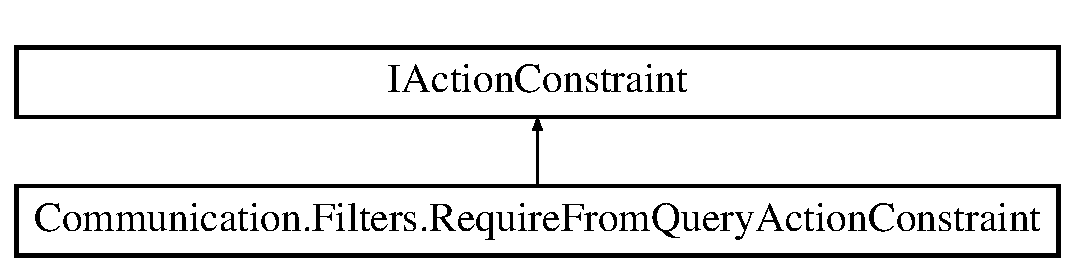
\includegraphics[height=2.000000cm]{class_communication_1_1_filters_1_1_require_from_query_action_constraint}
\end{center}
\end{figure}
\subsection*{Public Member Functions}
\begin{DoxyCompactItemize}
\item 
\mbox{\hyperlink{class_communication_1_1_filters_1_1_require_from_query_action_constraint_ac2fe17d4c55de254d83b1a896b5f3258}{Require\+From\+Query\+Action\+Constraint}} (string parameter)
\item 
bool \mbox{\hyperlink{class_communication_1_1_filters_1_1_require_from_query_action_constraint_a4d9bbad71f8e7c1708dde03e037e37db}{Accept}} (Action\+Constraint\+Context context)
\end{DoxyCompactItemize}
\subsection*{Public Attributes}
\begin{DoxyCompactItemize}
\item 
int \mbox{\hyperlink{class_communication_1_1_filters_1_1_require_from_query_action_constraint_aee1bc3b92237aade5ce159e2422df698}{Order}} =$>$ 999
\end{DoxyCompactItemize}


\subsection{Constructor \& Destructor Documentation}
\mbox{\Hypertarget{class_communication_1_1_filters_1_1_require_from_query_action_constraint_ac2fe17d4c55de254d83b1a896b5f3258}\label{class_communication_1_1_filters_1_1_require_from_query_action_constraint_ac2fe17d4c55de254d83b1a896b5f3258}} 
\index{Communication\+::\+Filters\+::\+Require\+From\+Query\+Action\+Constraint@{Communication\+::\+Filters\+::\+Require\+From\+Query\+Action\+Constraint}!Require\+From\+Query\+Action\+Constraint@{Require\+From\+Query\+Action\+Constraint}}
\index{Require\+From\+Query\+Action\+Constraint@{Require\+From\+Query\+Action\+Constraint}!Communication\+::\+Filters\+::\+Require\+From\+Query\+Action\+Constraint@{Communication\+::\+Filters\+::\+Require\+From\+Query\+Action\+Constraint}}
\subsubsection{\texorpdfstring{Require\+From\+Query\+Action\+Constraint()}{RequireFromQueryActionConstraint()}}
{\footnotesize\ttfamily Communication.\+Filters.\+Require\+From\+Query\+Action\+Constraint.\+Require\+From\+Query\+Action\+Constraint (\begin{DoxyParamCaption}\item[{string}]{parameter }\end{DoxyParamCaption})}



\subsection{Member Function Documentation}
\mbox{\Hypertarget{class_communication_1_1_filters_1_1_require_from_query_action_constraint_a4d9bbad71f8e7c1708dde03e037e37db}\label{class_communication_1_1_filters_1_1_require_from_query_action_constraint_a4d9bbad71f8e7c1708dde03e037e37db}} 
\index{Communication\+::\+Filters\+::\+Require\+From\+Query\+Action\+Constraint@{Communication\+::\+Filters\+::\+Require\+From\+Query\+Action\+Constraint}!Accept@{Accept}}
\index{Accept@{Accept}!Communication\+::\+Filters\+::\+Require\+From\+Query\+Action\+Constraint@{Communication\+::\+Filters\+::\+Require\+From\+Query\+Action\+Constraint}}
\subsubsection{\texorpdfstring{Accept()}{Accept()}}
{\footnotesize\ttfamily bool Communication.\+Filters.\+Require\+From\+Query\+Action\+Constraint.\+Accept (\begin{DoxyParamCaption}\item[{Action\+Constraint\+Context}]{context }\end{DoxyParamCaption})}



\subsection{Member Data Documentation}
\mbox{\Hypertarget{class_communication_1_1_filters_1_1_require_from_query_action_constraint_aee1bc3b92237aade5ce159e2422df698}\label{class_communication_1_1_filters_1_1_require_from_query_action_constraint_aee1bc3b92237aade5ce159e2422df698}} 
\index{Communication\+::\+Filters\+::\+Require\+From\+Query\+Action\+Constraint@{Communication\+::\+Filters\+::\+Require\+From\+Query\+Action\+Constraint}!Order@{Order}}
\index{Order@{Order}!Communication\+::\+Filters\+::\+Require\+From\+Query\+Action\+Constraint@{Communication\+::\+Filters\+::\+Require\+From\+Query\+Action\+Constraint}}
\subsubsection{\texorpdfstring{Order}{Order}}
{\footnotesize\ttfamily int Communication.\+Filters.\+Require\+From\+Query\+Action\+Constraint.\+Order =$>$ 999}



The documentation for this class was generated from the following file\+:\begin{DoxyCompactItemize}
\item 
Filters/\mbox{\hyperlink{_require_from_query_attribute_8cs}{Require\+From\+Query\+Attribute.\+cs}}\end{DoxyCompactItemize}

\hypertarget{class_communication_1_1_filters_1_1_require_from_query_attribute}{}\section{Communication.\+Filters.\+Require\+From\+Query\+Attribute Class Reference}
\label{class_communication_1_1_filters_1_1_require_from_query_attribute}\index{Communication.\+Filters.\+Require\+From\+Query\+Attribute@{Communication.\+Filters.\+Require\+From\+Query\+Attribute}}


Taken from\+: \href{https://www.strathweb.com/2016/09/required-query-string-parameters-in-asp-net-core-mvc/}{\tt https\+://www.\+strathweb.\+com/2016/09/required-\/query-\/string-\/parameters-\/in-\/asp-\/net-\/core-\/mvc/}  


Inheritance diagram for Communication.\+Filters.\+Require\+From\+Query\+Attribute\+:\begin{figure}[H]
\begin{center}
\leavevmode
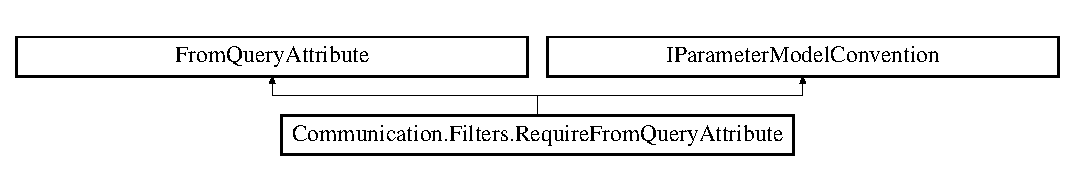
\includegraphics[height=1.848185cm]{class_communication_1_1_filters_1_1_require_from_query_attribute}
\end{center}
\end{figure}
\subsection*{Public Member Functions}
\begin{DoxyCompactItemize}
\item 
void \mbox{\hyperlink{class_communication_1_1_filters_1_1_require_from_query_attribute_aa627be8fe80705612e7c06b24ad34a59}{Apply}} (Parameter\+Model parameter)
\end{DoxyCompactItemize}


\subsection{Detailed Description}
Taken from\+: \href{https://www.strathweb.com/2016/09/required-query-string-parameters-in-asp-net-core-mvc/}{\tt https\+://www.\+strathweb.\+com/2016/09/required-\/query-\/string-\/parameters-\/in-\/asp-\/net-\/core-\/mvc/} 



\subsection{Member Function Documentation}
\mbox{\Hypertarget{class_communication_1_1_filters_1_1_require_from_query_attribute_aa627be8fe80705612e7c06b24ad34a59}\label{class_communication_1_1_filters_1_1_require_from_query_attribute_aa627be8fe80705612e7c06b24ad34a59}} 
\index{Communication\+::\+Filters\+::\+Require\+From\+Query\+Attribute@{Communication\+::\+Filters\+::\+Require\+From\+Query\+Attribute}!Apply@{Apply}}
\index{Apply@{Apply}!Communication\+::\+Filters\+::\+Require\+From\+Query\+Attribute@{Communication\+::\+Filters\+::\+Require\+From\+Query\+Attribute}}
\subsubsection{\texorpdfstring{Apply()}{Apply()}}
{\footnotesize\ttfamily void Communication.\+Filters.\+Require\+From\+Query\+Attribute.\+Apply (\begin{DoxyParamCaption}\item[{Parameter\+Model}]{parameter }\end{DoxyParamCaption})}



The documentation for this class was generated from the following file\+:\begin{DoxyCompactItemize}
\item 
Filters/\mbox{\hyperlink{_require_from_query_attribute_8cs}{Require\+From\+Query\+Attribute.\+cs}}\end{DoxyCompactItemize}

\hypertarget{class_communication_1_1_startup}{}\section{Communication.\+Startup Class Reference}
\label{class_communication_1_1_startup}\index{Communication.\+Startup@{Communication.\+Startup}}
\subsection*{Public Member Functions}
\begin{DoxyCompactItemize}
\item 
\mbox{\hyperlink{class_communication_1_1_startup_acbe360990f13465b22be5261abfa83e0}{Startup}} (I\+Configuration configuration)
\item 
void \mbox{\hyperlink{class_communication_1_1_startup_a9e95f261ac4022f8ccbde0579e88f5f8}{Configure\+Services}} (I\+Service\+Collection services)
\item 
void \mbox{\hyperlink{class_communication_1_1_startup_a7dc3e759d9ba10ab8c26c9194e211e3f}{Configure}} (I\+Application\+Builder app, I\+Hosting\+Environment env)
\end{DoxyCompactItemize}
\subsection*{Properties}
\begin{DoxyCompactItemize}
\item 
I\+Configuration \mbox{\hyperlink{class_communication_1_1_startup_af9e7ee914d5371b00bc7f755a63ca7df}{Configuration}}\hspace{0.3cm}{\ttfamily  \mbox{[}get\mbox{]}}
\end{DoxyCompactItemize}


\subsection{Constructor \& Destructor Documentation}
\mbox{\Hypertarget{class_communication_1_1_startup_acbe360990f13465b22be5261abfa83e0}\label{class_communication_1_1_startup_acbe360990f13465b22be5261abfa83e0}} 
\index{Communication\+::\+Startup@{Communication\+::\+Startup}!Startup@{Startup}}
\index{Startup@{Startup}!Communication\+::\+Startup@{Communication\+::\+Startup}}
\subsubsection{\texorpdfstring{Startup()}{Startup()}}
{\footnotesize\ttfamily Communication.\+Startup.\+Startup (\begin{DoxyParamCaption}\item[{I\+Configuration}]{configuration }\end{DoxyParamCaption})}



\subsection{Member Function Documentation}
\mbox{\Hypertarget{class_communication_1_1_startup_a7dc3e759d9ba10ab8c26c9194e211e3f}\label{class_communication_1_1_startup_a7dc3e759d9ba10ab8c26c9194e211e3f}} 
\index{Communication\+::\+Startup@{Communication\+::\+Startup}!Configure@{Configure}}
\index{Configure@{Configure}!Communication\+::\+Startup@{Communication\+::\+Startup}}
\subsubsection{\texorpdfstring{Configure()}{Configure()}}
{\footnotesize\ttfamily void Communication.\+Startup.\+Configure (\begin{DoxyParamCaption}\item[{I\+Application\+Builder}]{app,  }\item[{I\+Hosting\+Environment}]{env }\end{DoxyParamCaption})}

\mbox{\Hypertarget{class_communication_1_1_startup_a9e95f261ac4022f8ccbde0579e88f5f8}\label{class_communication_1_1_startup_a9e95f261ac4022f8ccbde0579e88f5f8}} 
\index{Communication\+::\+Startup@{Communication\+::\+Startup}!Configure\+Services@{Configure\+Services}}
\index{Configure\+Services@{Configure\+Services}!Communication\+::\+Startup@{Communication\+::\+Startup}}
\subsubsection{\texorpdfstring{Configure\+Services()}{ConfigureServices()}}
{\footnotesize\ttfamily void Communication.\+Startup.\+Configure\+Services (\begin{DoxyParamCaption}\item[{I\+Service\+Collection}]{services }\end{DoxyParamCaption})}



\subsection{Property Documentation}
\mbox{\Hypertarget{class_communication_1_1_startup_af9e7ee914d5371b00bc7f755a63ca7df}\label{class_communication_1_1_startup_af9e7ee914d5371b00bc7f755a63ca7df}} 
\index{Communication\+::\+Startup@{Communication\+::\+Startup}!Configuration@{Configuration}}
\index{Configuration@{Configuration}!Communication\+::\+Startup@{Communication\+::\+Startup}}
\subsubsection{\texorpdfstring{Configuration}{Configuration}}
{\footnotesize\ttfamily I\+Configuration Communication.\+Startup.\+Configuration\hspace{0.3cm}{\ttfamily [get]}}



The documentation for this class was generated from the following file\+:\begin{DoxyCompactItemize}
\item 
\mbox{\hyperlink{_startup_8cs}{Startup.\+cs}}\end{DoxyCompactItemize}

\hypertarget{class_communication_1_1_r_e_s_t_controllers_1_1_user_controller}{}\section{Communication.\+R\+E\+S\+T\+Controllers.\+User\+Controller Class Reference}
\label{class_communication_1_1_r_e_s_t_controllers_1_1_user_controller}\index{Communication.\+R\+E\+S\+T\+Controllers.\+User\+Controller@{Communication.\+R\+E\+S\+T\+Controllers.\+User\+Controller}}
Inheritance diagram for Communication.\+R\+E\+S\+T\+Controllers.\+User\+Controller\+:\begin{figure}[H]
\begin{center}
\leavevmode
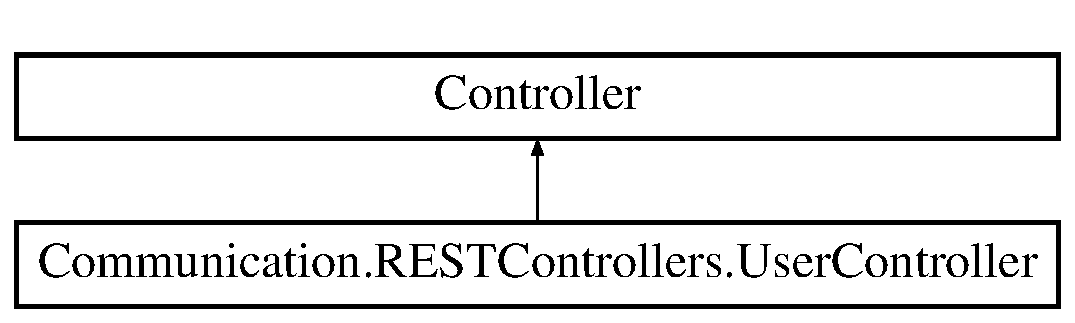
\includegraphics[height=2.000000cm]{class_communication_1_1_r_e_s_t_controllers_1_1_user_controller}
\end{center}
\end{figure}
\subsection*{Public Member Functions}
\begin{DoxyCompactItemize}
\item 
\mbox{\hyperlink{class_communication_1_1_r_e_s_t_controllers_1_1_user_controller_a5a4d1736034eb42ed3f6935923b3185c}{User\+Controller}} (I\+User\+Controller controller)
\item 
I\+Action\+Result \mbox{\hyperlink{class_communication_1_1_r_e_s_t_controllers_1_1_user_controller_a8a737663a9c771648976dd701cb10958}{Get\+User}} (\mbox{[}From\+Header\mbox{]} string username, \mbox{[}From\+Header\mbox{]} string password)
\item 
I\+Action\+Result \mbox{\hyperlink{class_communication_1_1_r_e_s_t_controllers_1_1_user_controller_a34eb238433f582672fa80aea7e830822}{Create\+User}} (\mbox{[}From\+Body\mbox{]} User raw\+User)
\item 
I\+Action\+Result \mbox{\hyperlink{class_communication_1_1_r_e_s_t_controllers_1_1_user_controller_aa97f36ee98608527aed8be3ffe27476f}{Update\+User}} (\mbox{[}From\+Header\mbox{]} string username, \mbox{[}From\+Body\mbox{]} User user)
\end{DoxyCompactItemize}


\subsection{Constructor \& Destructor Documentation}
\mbox{\Hypertarget{class_communication_1_1_r_e_s_t_controllers_1_1_user_controller_a5a4d1736034eb42ed3f6935923b3185c}\label{class_communication_1_1_r_e_s_t_controllers_1_1_user_controller_a5a4d1736034eb42ed3f6935923b3185c}} 
\index{Communication\+::\+R\+E\+S\+T\+Controllers\+::\+User\+Controller@{Communication\+::\+R\+E\+S\+T\+Controllers\+::\+User\+Controller}!User\+Controller@{User\+Controller}}
\index{User\+Controller@{User\+Controller}!Communication\+::\+R\+E\+S\+T\+Controllers\+::\+User\+Controller@{Communication\+::\+R\+E\+S\+T\+Controllers\+::\+User\+Controller}}
\subsubsection{\texorpdfstring{User\+Controller()}{UserController()}}
{\footnotesize\ttfamily Communication.\+R\+E\+S\+T\+Controllers.\+User\+Controller.\+User\+Controller (\begin{DoxyParamCaption}\item[{I\+User\+Controller}]{controller }\end{DoxyParamCaption})}



\subsection{Member Function Documentation}
\mbox{\Hypertarget{class_communication_1_1_r_e_s_t_controllers_1_1_user_controller_a34eb238433f582672fa80aea7e830822}\label{class_communication_1_1_r_e_s_t_controllers_1_1_user_controller_a34eb238433f582672fa80aea7e830822}} 
\index{Communication\+::\+R\+E\+S\+T\+Controllers\+::\+User\+Controller@{Communication\+::\+R\+E\+S\+T\+Controllers\+::\+User\+Controller}!Create\+User@{Create\+User}}
\index{Create\+User@{Create\+User}!Communication\+::\+R\+E\+S\+T\+Controllers\+::\+User\+Controller@{Communication\+::\+R\+E\+S\+T\+Controllers\+::\+User\+Controller}}
\subsubsection{\texorpdfstring{Create\+User()}{CreateUser()}}
{\footnotesize\ttfamily I\+Action\+Result Communication.\+R\+E\+S\+T\+Controllers.\+User\+Controller.\+Create\+User (\begin{DoxyParamCaption}\item[{\mbox{[}\+From\+Body\mbox{]} User}]{raw\+User }\end{DoxyParamCaption})}

\mbox{\Hypertarget{class_communication_1_1_r_e_s_t_controllers_1_1_user_controller_a8a737663a9c771648976dd701cb10958}\label{class_communication_1_1_r_e_s_t_controllers_1_1_user_controller_a8a737663a9c771648976dd701cb10958}} 
\index{Communication\+::\+R\+E\+S\+T\+Controllers\+::\+User\+Controller@{Communication\+::\+R\+E\+S\+T\+Controllers\+::\+User\+Controller}!Get\+User@{Get\+User}}
\index{Get\+User@{Get\+User}!Communication\+::\+R\+E\+S\+T\+Controllers\+::\+User\+Controller@{Communication\+::\+R\+E\+S\+T\+Controllers\+::\+User\+Controller}}
\subsubsection{\texorpdfstring{Get\+User()}{GetUser()}}
{\footnotesize\ttfamily I\+Action\+Result Communication.\+R\+E\+S\+T\+Controllers.\+User\+Controller.\+Get\+User (\begin{DoxyParamCaption}\item[{\mbox{[}\+From\+Header\mbox{]} string}]{username,  }\item[{\mbox{[}\+From\+Header\mbox{]} string}]{password }\end{DoxyParamCaption})}

\mbox{\Hypertarget{class_communication_1_1_r_e_s_t_controllers_1_1_user_controller_aa97f36ee98608527aed8be3ffe27476f}\label{class_communication_1_1_r_e_s_t_controllers_1_1_user_controller_aa97f36ee98608527aed8be3ffe27476f}} 
\index{Communication\+::\+R\+E\+S\+T\+Controllers\+::\+User\+Controller@{Communication\+::\+R\+E\+S\+T\+Controllers\+::\+User\+Controller}!Update\+User@{Update\+User}}
\index{Update\+User@{Update\+User}!Communication\+::\+R\+E\+S\+T\+Controllers\+::\+User\+Controller@{Communication\+::\+R\+E\+S\+T\+Controllers\+::\+User\+Controller}}
\subsubsection{\texorpdfstring{Update\+User()}{UpdateUser()}}
{\footnotesize\ttfamily I\+Action\+Result Communication.\+R\+E\+S\+T\+Controllers.\+User\+Controller.\+Update\+User (\begin{DoxyParamCaption}\item[{\mbox{[}\+From\+Header\mbox{]} string}]{username,  }\item[{\mbox{[}\+From\+Body\mbox{]} User}]{user }\end{DoxyParamCaption})}



The documentation for this class was generated from the following file\+:\begin{DoxyCompactItemize}
\item 
R\+E\+S\+T\+Controllers/\mbox{\hyperlink{_user_controller_8cs}{User\+Controller.\+cs}}\end{DoxyCompactItemize}

\hypertarget{class_communication_1_1_filters_1_1_validate_model_state_attribute}{}\section{Communication.\+Filters.\+Validate\+Model\+State\+Attribute Class Reference}
\label{class_communication_1_1_filters_1_1_validate_model_state_attribute}\index{Communication.\+Filters.\+Validate\+Model\+State\+Attribute@{Communication.\+Filters.\+Validate\+Model\+State\+Attribute}}
Inheritance diagram for Communication.\+Filters.\+Validate\+Model\+State\+Attribute\+:\begin{figure}[H]
\begin{center}
\leavevmode
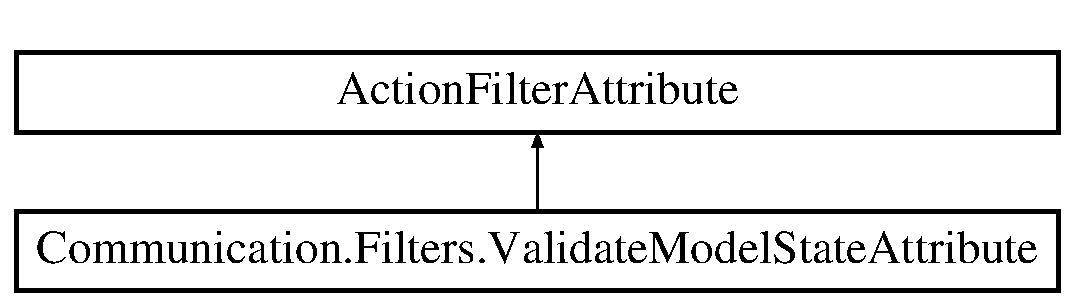
\includegraphics[height=2.000000cm]{class_communication_1_1_filters_1_1_validate_model_state_attribute}
\end{center}
\end{figure}
\subsection*{Public Member Functions}
\begin{DoxyCompactItemize}
\item 
override void \mbox{\hyperlink{class_communication_1_1_filters_1_1_validate_model_state_attribute_a785e43025a598082a88cb8a1ec43173b}{On\+Action\+Executing}} (Action\+Executing\+Context context)
\end{DoxyCompactItemize}


\subsection{Member Function Documentation}
\mbox{\Hypertarget{class_communication_1_1_filters_1_1_validate_model_state_attribute_a785e43025a598082a88cb8a1ec43173b}\label{class_communication_1_1_filters_1_1_validate_model_state_attribute_a785e43025a598082a88cb8a1ec43173b}} 
\index{Communication\+::\+Filters\+::\+Validate\+Model\+State\+Attribute@{Communication\+::\+Filters\+::\+Validate\+Model\+State\+Attribute}!On\+Action\+Executing@{On\+Action\+Executing}}
\index{On\+Action\+Executing@{On\+Action\+Executing}!Communication\+::\+Filters\+::\+Validate\+Model\+State\+Attribute@{Communication\+::\+Filters\+::\+Validate\+Model\+State\+Attribute}}
\subsubsection{\texorpdfstring{On\+Action\+Executing()}{OnActionExecuting()}}
{\footnotesize\ttfamily override void Communication.\+Filters.\+Validate\+Model\+State\+Attribute.\+On\+Action\+Executing (\begin{DoxyParamCaption}\item[{Action\+Executing\+Context}]{context }\end{DoxyParamCaption})}



The documentation for this class was generated from the following file\+:\begin{DoxyCompactItemize}
\item 
Filters/\mbox{\hyperlink{_validate_model_state_attribute_8cs}{Validate\+Model\+State\+Attribute.\+cs}}\end{DoxyCompactItemize}

\chapter{File Documentation}
\hypertarget{_authorization_swag_attribute_8cs}{}\section{Filters/\+Authorization\+Swag\+Attribute.cs File Reference}
\label{_authorization_swag_attribute_8cs}\index{Filters/\+Authorization\+Swag\+Attribute.\+cs@{Filters/\+Authorization\+Swag\+Attribute.\+cs}}
\subsection*{Classes}
\begin{DoxyCompactItemize}
\item 
class \mbox{\hyperlink{class_communication_1_1_filters_1_1_authorization_swag_attribute}{Communication.\+Filters.\+Authorization\+Swag\+Attribute}}
\begin{DoxyCompactList}\small\item\em Provides authentication for requests for Swag Api. Reads username and password from the header of the Http\+Request \end{DoxyCompactList}\end{DoxyCompactItemize}
\subsection*{Namespaces}
\begin{DoxyCompactItemize}
\item 
namespace \mbox{\hyperlink{namespace_communication_1_1_filters}{Communication.\+Filters}}
\end{DoxyCompactItemize}

\hypertarget{_require_from_query_attribute_8cs}{}\section{Filters/\+Require\+From\+Query\+Attribute.cs File Reference}
\label{_require_from_query_attribute_8cs}\index{Filters/\+Require\+From\+Query\+Attribute.\+cs@{Filters/\+Require\+From\+Query\+Attribute.\+cs}}
\subsection*{Classes}
\begin{DoxyCompactItemize}
\item 
class \mbox{\hyperlink{class_communication_1_1_filters_1_1_require_from_query_attribute}{Communication.\+Filters.\+Require\+From\+Query\+Attribute}}
\begin{DoxyCompactList}\small\item\em Taken from\+: \href{https://www.strathweb.com/2016/09/required-query-string-parameters-in-asp-net-core-mvc/}{\tt https\+://www.\+strathweb.\+com/2016/09/required-\/query-\/string-\/parameters-\/in-\/asp-\/net-\/core-\/mvc/} \end{DoxyCompactList}\item 
class \mbox{\hyperlink{class_communication_1_1_filters_1_1_require_from_query_action_constraint}{Communication.\+Filters.\+Require\+From\+Query\+Action\+Constraint}}
\end{DoxyCompactItemize}
\subsection*{Namespaces}
\begin{DoxyCompactItemize}
\item 
namespace \mbox{\hyperlink{namespace_communication_1_1_filters}{Communication.\+Filters}}
\end{DoxyCompactItemize}

\hypertarget{_validate_model_state_attribute_8cs}{}\section{Filters/\+Validate\+Model\+State\+Attribute.cs File Reference}
\label{_validate_model_state_attribute_8cs}\index{Filters/\+Validate\+Model\+State\+Attribute.\+cs@{Filters/\+Validate\+Model\+State\+Attribute.\+cs}}
\subsection*{Classes}
\begin{DoxyCompactItemize}
\item 
class \mbox{\hyperlink{class_communication_1_1_filters_1_1_validate_model_state_attribute}{Communication.\+Filters.\+Validate\+Model\+State\+Attribute}}
\end{DoxyCompactItemize}
\subsection*{Namespaces}
\begin{DoxyCompactItemize}
\item 
namespace \mbox{\hyperlink{namespace_communication_1_1_filters}{Communication.\+Filters}}
\end{DoxyCompactItemize}

\hypertarget{_json_input_formatter_8cs}{}\section{Formatters/\+Json\+Input\+Formatter.cs File Reference}
\label{_json_input_formatter_8cs}\index{Formatters/\+Json\+Input\+Formatter.\+cs@{Formatters/\+Json\+Input\+Formatter.\+cs}}
\subsection*{Classes}
\begin{DoxyCompactItemize}
\item 
class \mbox{\hyperlink{class_communication_1_1_formatters_1_1_json_input_formatter}{Communication.\+Formatters.\+Json\+Input\+Formatter}}
\end{DoxyCompactItemize}
\subsection*{Namespaces}
\begin{DoxyCompactItemize}
\item 
namespace \mbox{\hyperlink{namespace_communication_1_1_formatters}{Communication.\+Formatters}}
\end{DoxyCompactItemize}

\hypertarget{_i_lobby_controller_8cs}{}\section{Interfaces/\+I\+Lobby\+Controller.cs File Reference}
\label{_i_lobby_controller_8cs}\index{Interfaces/\+I\+Lobby\+Controller.\+cs@{Interfaces/\+I\+Lobby\+Controller.\+cs}}
\subsection*{Classes}
\begin{DoxyCompactItemize}
\item 
interface \mbox{\hyperlink{interface_application_1_1_interfaces_1_1_i_lobby_controller}{Application.\+Interfaces.\+I\+Lobby\+Controller}}
\end{DoxyCompactItemize}
\subsection*{Namespaces}
\begin{DoxyCompactItemize}
\item 
namespace \mbox{\hyperlink{namespace_application_1_1_interfaces}{Application.\+Interfaces}}
\end{DoxyCompactItemize}

\hypertarget{_utility_8cs}{}\section{Json\+Serializer\+Extensions/\+Utility.cs File Reference}
\label{_utility_8cs}\index{Json\+Serializer\+Extensions/\+Utility.\+cs@{Json\+Serializer\+Extensions/\+Utility.\+cs}}
\subsection*{Classes}
\begin{DoxyCompactItemize}
\item 
class {\bfseries Communication.\+Json\+Serializer\+Extensions.\+Utility}
\end{DoxyCompactItemize}
\subsection*{Namespaces}
\begin{DoxyCompactItemize}
\item 
namespace \mbox{\hyperlink{namespace_communication_1_1_json_serializer_extensions}{Communication.\+Json\+Serializer\+Extensions}}
\end{DoxyCompactItemize}

\hypertarget{_from_swag_dto_attribute_8cs}{}\section{Model\+Binders(Deprecated)/\+Attributes/\+From\+Swag\+Dto\+Attribute.cs File Reference}
\label{_from_swag_dto_attribute_8cs}\index{Model\+Binders(\+Deprecated)/\+Attributes/\+From\+Swag\+Dto\+Attribute.\+cs@{Model\+Binders(\+Deprecated)/\+Attributes/\+From\+Swag\+Dto\+Attribute.\+cs}}
\subsection*{Classes}
\begin{DoxyCompactItemize}
\item 
class \mbox{\hyperlink{class_communication_1_1_model_binders_1_1_attributes_1_1_from_swag_dto_attribute}{Communication.\+Model\+Binders.\+Attributes.\+From\+Swag\+Dto\+Attribute}}
\end{DoxyCompactItemize}
\subsection*{Namespaces}
\begin{DoxyCompactItemize}
\item 
namespace \mbox{\hyperlink{namespace_communication_1_1_model_binders_1_1_attributes}{Communication.\+Model\+Binders.\+Attributes}}
\end{DoxyCompactItemize}

\hypertarget{_i_from_swag_dto_attribute_8cs}{}\section{Model\+Binders(Deprecated)/\+Attributes/\+I\+From\+Swag\+Dto\+Attribute.cs File Reference}
\label{_i_from_swag_dto_attribute_8cs}\index{Model\+Binders(\+Deprecated)/\+Attributes/\+I\+From\+Swag\+Dto\+Attribute.\+cs@{Model\+Binders(\+Deprecated)/\+Attributes/\+I\+From\+Swag\+Dto\+Attribute.\+cs}}
\subsection*{Classes}
\begin{DoxyCompactItemize}
\item 
interface \mbox{\hyperlink{interface_communication_1_1_model_binders_1_1_attributes_1_1_i_from_swag_dto_attribute}{Communication.\+Model\+Binders.\+Attributes.\+I\+From\+Swag\+Dto\+Attribute}}
\end{DoxyCompactItemize}
\subsection*{Namespaces}
\begin{DoxyCompactItemize}
\item 
namespace \mbox{\hyperlink{namespace_communication_1_1_model_binders_1_1_attributes}{Communication.\+Model\+Binders.\+Attributes}}
\end{DoxyCompactItemize}

\hypertarget{_from_swag_dto_model_binder_8cs}{}\section{Model\+Binders(Deprecated)/\+From\+Swag\+Dto\+Model\+Binder.cs File Reference}
\label{_from_swag_dto_model_binder_8cs}\index{Model\+Binders(\+Deprecated)/\+From\+Swag\+Dto\+Model\+Binder.\+cs@{Model\+Binders(\+Deprecated)/\+From\+Swag\+Dto\+Model\+Binder.\+cs}}
\subsection*{Classes}
\begin{DoxyCompactItemize}
\item 
class \mbox{\hyperlink{class_communication_1_1_model_binders_1_1_from_swag_dto_model_binder}{Communication.\+Model\+Binders.\+From\+Swag\+Dto\+Model\+Binder}}
\begin{DoxyCompactList}\small\item\em Dto to Model converter and binder. The model will bind to the \char`\"{}value\char`\"{} part of a \char`\"{}auth\char`\"{}/\char`\"{}val\char`\"{} request as in accordance with Swag\+Attack Standards \end{DoxyCompactList}\end{DoxyCompactItemize}
\subsection*{Namespaces}
\begin{DoxyCompactItemize}
\item 
namespace \mbox{\hyperlink{namespace_communication_1_1_model_binders}{Communication.\+Model\+Binders}}
\end{DoxyCompactItemize}

\hypertarget{_from_dto_value_provider_8cs}{}\section{Model\+Binders(Deprecated)/\+Value\+Providers/\+From\+Dto\+Value\+Provider.cs File Reference}
\label{_from_dto_value_provider_8cs}\index{Model\+Binders(\+Deprecated)/\+Value\+Providers/\+From\+Dto\+Value\+Provider.\+cs@{Model\+Binders(\+Deprecated)/\+Value\+Providers/\+From\+Dto\+Value\+Provider.\+cs}}
\subsection*{Classes}
\begin{DoxyCompactItemize}
\item 
class \mbox{\hyperlink{class_communication_1_1_model_binders_1_1_value_providers_1_1_from_dto_value_provider}{Communication.\+Model\+Binders.\+Value\+Providers.\+From\+Dto\+Value\+Provider}}
\end{DoxyCompactItemize}
\subsection*{Namespaces}
\begin{DoxyCompactItemize}
\item 
namespace \mbox{\hyperlink{namespace_communication_1_1_model_binders_1_1_value_providers}{Communication.\+Model\+Binders.\+Value\+Providers}}
\end{DoxyCompactItemize}

\hypertarget{_from_dto_value_provider_factory_8cs}{}\section{Model\+Binders(Deprecated)/\+Value\+Providers/\+From\+Dto\+Value\+Provider\+Factory.cs File Reference}
\label{_from_dto_value_provider_factory_8cs}\index{Model\+Binders(\+Deprecated)/\+Value\+Providers/\+From\+Dto\+Value\+Provider\+Factory.\+cs@{Model\+Binders(\+Deprecated)/\+Value\+Providers/\+From\+Dto\+Value\+Provider\+Factory.\+cs}}
\subsection*{Classes}
\begin{DoxyCompactItemize}
\item 
class \mbox{\hyperlink{class_communication_1_1_model_binders_1_1_value_providers_1_1_from_dto_value_provider_factory}{Communication.\+Model\+Binders.\+Value\+Providers.\+From\+Dto\+Value\+Provider\+Factory}}
\end{DoxyCompactItemize}
\subsection*{Namespaces}
\begin{DoxyCompactItemize}
\item 
namespace \mbox{\hyperlink{namespace_communication_1_1_model_binders_1_1_value_providers}{Communication.\+Model\+Binders.\+Value\+Providers}}
\end{DoxyCompactItemize}

\hypertarget{_debug_2netcoreapp2_80_2_communication_8_assembly_info_8cs}{}\section{obj/\+Debug/netcoreapp2.0/\+Communication.Assembly\+Info.\+cs File Reference}
\label{_debug_2netcoreapp2_80_2_communication_8_assembly_info_8cs}\index{obj/\+Debug/netcoreapp2.\+0/\+Communication.\+Assembly\+Info.\+cs@{obj/\+Debug/netcoreapp2.\+0/\+Communication.\+Assembly\+Info.\+cs}}

\hypertarget{_release_2netcoreapp2_80_2_communication_8_assembly_info_8cs}{}\section{obj/\+Release/netcoreapp2.0/\+Communication.Assembly\+Info.\+cs File Reference}
\label{_release_2netcoreapp2_80_2_communication_8_assembly_info_8cs}\index{obj/\+Release/netcoreapp2.\+0/\+Communication.\+Assembly\+Info.\+cs@{obj/\+Release/netcoreapp2.\+0/\+Communication.\+Assembly\+Info.\+cs}}

\hypertarget{_program_8cs}{}\section{Program.\+cs File Reference}
\label{_program_8cs}\index{Program.\+cs@{Program.\+cs}}
\subsection*{Classes}
\begin{DoxyCompactItemize}
\item 
class \mbox{\hyperlink{class_communication_1_1_program}{Communication.\+Program}}
\end{DoxyCompactItemize}
\subsection*{Namespaces}
\begin{DoxyCompactItemize}
\item 
namespace \mbox{\hyperlink{namespace_communication}{Communication}}
\end{DoxyCompactItemize}

\hypertarget{_lobby_controller_8cs}{}\section{R\+E\+S\+T\+Controllers/\+Lobby\+Controller.cs File Reference}
\label{_lobby_controller_8cs}\index{R\+E\+S\+T\+Controllers/\+Lobby\+Controller.\+cs@{R\+E\+S\+T\+Controllers/\+Lobby\+Controller.\+cs}}
\subsection*{Classes}
\begin{DoxyCompactItemize}
\item 
class \mbox{\hyperlink{class_communication_1_1_r_e_s_t_controllers_1_1_lobby_controller}{Communication.\+R\+E\+S\+T\+Controllers.\+Lobby\+Controller}}
\end{DoxyCompactItemize}
\subsection*{Namespaces}
\begin{DoxyCompactItemize}
\item 
namespace \mbox{\hyperlink{namespace_communication_1_1_r_e_s_t_controllers}{Communication.\+R\+E\+S\+T\+Controllers}}
\end{DoxyCompactItemize}

\hypertarget{_user_controller_8cs}{}\section{Controllers/\+User\+Controller.cs File Reference}
\label{_user_controller_8cs}\index{Controllers/\+User\+Controller.\+cs@{Controllers/\+User\+Controller.\+cs}}
\subsection*{Classes}
\begin{DoxyCompactItemize}
\item 
class \mbox{\hyperlink{class_application_1_1_controllers_1_1_user_controller}{Application.\+Controllers.\+User\+Controller}}
\begin{DoxyCompactList}\small\item\em \mbox{\hyperlink{namespace_application}{Application}} User Controller The main purpose of this class is to decouple the framework from our application logic \end{DoxyCompactList}\end{DoxyCompactItemize}
\subsection*{Namespaces}
\begin{DoxyCompactItemize}
\item 
namespace \mbox{\hyperlink{namespace_application_1_1_controllers}{Application.\+Controllers}}
\end{DoxyCompactItemize}

\hypertarget{_startup_8cs}{}\section{Startup.\+cs File Reference}
\label{_startup_8cs}\index{Startup.\+cs@{Startup.\+cs}}
\subsection*{Classes}
\begin{DoxyCompactItemize}
\item 
class \mbox{\hyperlink{class_communication_1_1_startup}{Communication.\+Startup}}
\end{DoxyCompactItemize}
\subsection*{Namespaces}
\begin{DoxyCompactItemize}
\item 
namespace \mbox{\hyperlink{namespace_communication}{Communication}}
\end{DoxyCompactItemize}

%--- End generated contents ---

% Index
\backmatter
\newpage
\phantomsection
\clearemptydoublepage
\addcontentsline{toc}{chapter}{Index}
\printindex

\end{document}
